% Options for packages loaded elsewhere
\PassOptionsToPackage{unicode}{hyperref}
\PassOptionsToPackage{hyphens}{url}
\PassOptionsToPackage{dvipsnames,svgnames,x11names}{xcolor}
%
\documentclass[
  12pt,
  a4paper, twoside]{book}
\usepackage{amsmath,amssymb}
\usepackage{iftex}
\ifPDFTeX
  \usepackage[T1]{fontenc}
  \usepackage[utf8]{inputenc}
  \usepackage{textcomp} % provide euro and other symbols
\else % if luatex or xetex
  \usepackage{unicode-math} % this also loads fontspec
  \defaultfontfeatures{Scale=MatchLowercase}
  \defaultfontfeatures[\rmfamily]{Ligatures=TeX,Scale=1}
\fi
\usepackage{lmodern}
\ifPDFTeX\else
  % xetex/luatex font selection
\fi
% Use upquote if available, for straight quotes in verbatim environments
\IfFileExists{upquote.sty}{\usepackage{upquote}}{}
\IfFileExists{microtype.sty}{% use microtype if available
  \usepackage[]{microtype}
  \UseMicrotypeSet[protrusion]{basicmath} % disable protrusion for tt fonts
}{}
\makeatletter
\@ifundefined{KOMAClassName}{% if non-KOMA class
  \IfFileExists{parskip.sty}{%
    \usepackage{parskip}
  }{% else
    \setlength{\parindent}{0pt}
    \setlength{\parskip}{6pt plus 2pt minus 1pt}}
}{% if KOMA class
  \KOMAoptions{parskip=half}}
\makeatother
\usepackage{xcolor}
\usepackage{longtable,booktabs,array}
\usepackage{calc} % for calculating minipage widths
% Correct order of tables after \paragraph or \subparagraph
\usepackage{etoolbox}
\makeatletter
\patchcmd\longtable{\par}{\if@noskipsec\mbox{}\fi\par}{}{}
\makeatother
% Allow footnotes in longtable head/foot
\IfFileExists{footnotehyper.sty}{\usepackage{footnotehyper}}{\usepackage{footnote}}
\makesavenoteenv{longtable}
\usepackage{graphicx}
\makeatletter
\def\maxwidth{\ifdim\Gin@nat@width>\linewidth\linewidth\else\Gin@nat@width\fi}
\def\maxheight{\ifdim\Gin@nat@height>\textheight\textheight\else\Gin@nat@height\fi}
\makeatother
% Scale images if necessary, so that they will not overflow the page
% margins by default, and it is still possible to overwrite the defaults
% using explicit options in \includegraphics[width, height, ...]{}
\setkeys{Gin}{width=\maxwidth,height=\maxheight,keepaspectratio}
% Set default figure placement to htbp
\makeatletter
\def\fps@figure{htbp}
\makeatother
\setlength{\emergencystretch}{3em} % prevent overfull lines
\providecommand{\tightlist}{%
  \setlength{\itemsep}{0pt}\setlength{\parskip}{0pt}}
\setcounter{secnumdepth}{5}
\ifLuaTeX
\usepackage[bidi=basic]{babel}
\else
\usepackage[bidi=default]{babel}
\fi
\babelprovide[main,import]{finnish}
% get rid of language-specific shorthands (see #6817):
\let\LanguageShortHands\languageshorthands
\def\languageshorthands#1{}
\usepackage{booktabs}
\usepackage[T1]{fontenc}
\usepackage{color}
\usepackage{xspace}
\usepackage{tikz-cd}
\usepackage{mathtools}
\usepackage{mathrsfs}
\usepackage{comment}
\usepackage{commath}
\usepackage{pict2e}
\usepackage{float}
\usepackage{array, makecell}
\usepackage{amsthm}														% 
\usepackage{amsmath}
%\usepackage[tagpdf]{axessibility} 
\usepackage[ruled,vlined,shortend]{algorithm2e} 
\usepackage{graphicx}
\usepackage{multicol}
\usepackage{gensymb}
%\usepackage[a-3b]{pdfx}
\graphicspath{ {./images/} }
\usetikzlibrary{shapes.geometric,arrows}
\def\TikZ{Ti\emph{k}Z\ }
\renewcommand{\algorithmcfname}{Algoritmi}
\usepackage{babel}
  \addto{\captionsfinnish}{\renewcommand{\bibname}{Lähteet}}
\usepackage{geometry}
\geometry{
    a4paper,
    total={150mm,237mm},
    left=30mm,
    top=30mm,
    }
\usepackage[numbers]{natbib}
\newcommand{\tekija}{{Lasse Rintakumpu}}
\newcommand{\titteli}{{}} 
\newcommand{\otsikko}{{Hiukassuodin- ja hiukassiloitinalgoritmit sekä niiden soveltaminen AoA-menetelmään perustuvassa Bluetooth-sisätilapaikannuksessa}} 
\newcommand{\tutkielma}{{Pro gradu }}
\newcommand{\aika}{{Maaliskuu 2024}} 
\newcommand{\paaaine}{{Tilastotiede}} 
\newcommand{\ohjaaja}{{Ohjaajan titteli (Prof./Dos./FT) ja nimi }} %
\newcommand{\tarkastaja}{{Toisen tarkastajan titteli (Prof./Dos./FT) ja nimi}} 
\ifLuaTeX
  \usepackage{selnolig}  % disable illegal ligatures
\fi
\usepackage[]{natbib}
\bibliographystyle{plainnat}
\IfFileExists{bookmark.sty}{\usepackage{bookmark}}{\usepackage{hyperref}}
\IfFileExists{xurl.sty}{\usepackage{xurl}}{} % add URL line breaks if available
\urlstyle{same}
\hypersetup{
  pdflang={fi},
  colorlinks=true,
  linkcolor={blue},
  filecolor={Maroon},
  citecolor={blue},
  urlcolor={blue},
  pdfcreator={LaTeX via pandoc}}

\author{}
\date{\vspace{-2.5em}}

\begin{document}

\pagenumbering{roman}
\pagestyle{empty}

\begin{center}

\includegraphics[width=10cm]{UTU_logo_FI}
\end{center}

\vspace{3.0cm}
\begin{center}\large
{\sc \otsikko} 
\end{center}

\vspace{0.5cm}
\begin{center}
\titteli \tekija
\end{center}

\vspace{0.5cm}
\begin{center}
\tutkielma -tutkielma\\
\aika
\end{center}

\vspace{2.5cm}
\begin{center}
\begin{tabular}{l}
Tarkastajat:\\
\ohjaaja \\
\tarkastaja
\end{tabular}
\end{center}

\vspace{2.5cm}
\begin{center}
MATEMATIIKAN JA TILASTOTIETEEN LAITOS
\end{center}

\newpage\null

\vspace{22cm}

\noindent Turun yliopiston laatujärjestelmän mukaisesti tämän julkaisun alkuperäisyys on tarkastettu Turnitin OriginalityCheck-järjestelmällä

\cleardoublepage

\noindent
TURUN YLIOPISTO \newline
Matematiikan ja tilastotieteen laitos\newline

\noindent \textsc{\tekija}: \otsikko \newline
\tutkielma-tutkielma, X s. \newline
\paaaine \newline
\aika
\par\noindent{\rule{\textwidth}{.2mm}} \newline


\vspace{4mm}\noindent Tutkielmassa esitetään hiukassuodin- ja hiukassiloitinalgoritmien teoria Bayesilaisessa tilastotieteellisessä viitekehyksessä. Lisäksi tutkielmassa käsitellään hiukassuotimien varianssin estimointia.

\vspace{4mm}\noindent Empiirisenä esimerkkinä tutkielmassa tarkastellaan hiukassuodin- ja hiukassiloitinalgoritmien käyttöä AoA-teknologiaan perustuvassa Bluetooth-sisätilapaikannusratkaisussa.

\vspace{4mm}\noindent Asiasanat: SMC-menetelmät, Monte Carlo -menetelmät, sekventiaalinen Monte Carlo, suodinongelma, hiukassuodin, hiukassiloitin, SIR-algoritmi, sisätilapaikannus, BLE, AoA, triangulaatio, Bayesilainen päättely

\cleardoublepage

\cleardoublepage

\pagestyle{plain} 
\pagenumbering{arabic} 

{
\hypersetup{linkcolor=blue}
\setcounter{tocdepth}{2}
\tableofcontents
}
\setlength\parindent{24pt}
\setlength\parskip{3pt}

\chapter{Johdanto}

Hiukassuotimet ovat joukko Monte Carlo -algoritmeja, joiden avulla voidaan ratkaista ns. suodinongelma, kun ongelma on epälineaarinen ja/tai ongelmaan liittyvä kohina ei noudata normaalijakaumaa. Hiukassuotimille on lukuisia sovellutuksia esimerkiksi Bayesilaisessa tilastotieteessä, fysiikassa ja robotiikassa.

Tämän tutkielman tavoitteena on esittää hiukassuotimien teoria sekä joitakin menetelmäperheeseen kuuluvia algoritmeja. Tutkielman ensimmäisessä luvussa kuvataan yleisellä tasolla sekä suodinongelma että sen ratkaisujen historiaa ja esitetään joitakin Monte Carlo -menetelmiin liittyviä yleisiä tuloksia sekä Bayesilainen viitekehys suodinongelmalle. Toisessa luvussa kuvataan kaksi hiukassuodinalgoritmia, saapasremmisuodin sekä SIR-algoritmi ja perehdytään hiukassuotimen varianssin estimointiin. Kolmannessa luvussa tarkastellaan suodinongelmaan läheisesti liittyvää siloitteluongelma ja esitetään hiukassiloitinalgoritmeja tämän ongelman ratkaisemiseksi. Neljäs luku keskittyy hiukassuotimen käyttöön empiirisessä AoA/Bluetooth-teknologiaan perustuvassa sisätilapaikannussovelluksessa. Tässä luvussa esitetään myös hiukassuodinalgoritmit radiosignaalin tulokulman arviointiin sekä radiovastaanottimen kalibrointiin. Lisäksi käsitellään lyhyesti sisätilapaikannuksessa hyödynnettävää karttasovitusalgoritmia.

Hiukassuodin- sekä hiukassiloitinalgoritmien osalta tutkielman esitykset seuraavat erityisesti Simo Särkän kirjaa \textit{Bayesian Filtering and Smoothing} (2013) \citep{sarkka-2013}, Fredrik Gustafssonin artikkelia ``Particle Filter Theory and Practice with Positioning Applications'' (2010) \citep{gustafsson-2010} sekä Olivier Cappén, Simon J. Godsillin ja Eric Moulines'n artikkelia ``An overview of existing methods and recent advances in sequential Monte Carlo'' (2007) \citep{cappe-2007}. Hiukassuotimien varianssin estimointi seuraa artikkeleita TODO.

\section{Notaatioista}

Tässä tutkielmassa käytetään seuraavia notaatioita. Vektoreita merkitään pienellä kirjaimella, esimerkiksi \(z\). Hiukassuotimen hiukkaset sisältäviä vektoreita merkitään \(x_k^i\), missä alaindeksi viittaa ajanhetkeen \(k, k=\{1,\ldots,T\}\) ja yläindeksi partikkeliin \(i\), missä \(i=\{1,\ldots,N\}\). Ajanhetkien \(k, k=\{1,\ldots,T\}\) havainnot sisältäviä vektoreita merkitään \(\{y_1,\ldots,y_k\}\). Lähtökohtaisesti kaikki tutkielmassa esitetyt muuttujat ovat ylä- ja alaindeksejä lukuunottamattavektoreita. Skalaareihin pyritään viittaamaan isoilla kirjaimilla, esimerkiksi \(Z\). Milloin tämä ei ole mahdollista, selviää muuttujan skalaariarvoisuus asiayhtedestä. Prosesseihin viitataan alaindeksoidulla isolla kirjaimella, esimerkiksi \(X_k\). Matriiseja merkitään isolla lihavoidulla kirjaimella, esimerkiksi \(\mathbf{X}\) ja funktiota TODO. Taulukossa \ref{tab:lyhenteet-ja-symbolit} esitetään tutkielman keskeisimmät lyhenteet ja symbolit.

\begin{table}

\caption{\label{tab:lyhenteet-ja-symbolit}Lyhenteet ja symbolit}
\centering
\begin{tabular}[t]{ll}
\toprule
Lyhenne tai symboli & Selitys\\
\midrule
RTSS & \textit{Rauch-Turn-Striebel smoother}, Rauch-Turn-Striebel-siloitin\\
SMC & \makecell[l]{\textit{Sequential Monte Carlo}, \\sekventiaalinen Monte Carlo -menetelmä, \\synonyymi hiukassuotimelle}\\
BS-PS & \textit{Backwards simulation particle smoother}\\
\bottomrule
\end{tabular}
\end{table}

\section{Suodinongelma}

Stokastisten prosessien teoriassa suodinongelmaksi kutsutaan tilannetta, jossa halutaan muodostaa keskineliövirheen mielessä paras mahdollinen estimaatti jonkin järjestelmän tilan arvoille, kun ainoastaan osa tiloista voidaan havaita ja/tai havaintoihin liittyy kohinaa. Tavoitteena on toisin sanoen laskea jonkin prosessin posteriorijakauma kyseisten havaintojen perusteella. Ongelmaa havainnollistaa kaavio (\ref{mallikaavio}).

\begin{equation}\label{mallikaavio}
\begin{tikzcd}
x_1 \arrow[d] \arrow[r] & x_2 \arrow[d] \arrow[r] & x_3 \arrow[d] \arrow[r] & \ldots & \makebox[\widthof{$ \text{havainnot}$}]{$\text{piilossa olevat tilat}$} \\
y_1  & y_2  & y_3  & \ldots & \makebox[\widthof{$ \text{havainnot}$}]{$\text{havainnot}$}
\end{tikzcd}
\end{equation}

Tässä tutkielmassa keskitytään erityisesti epälineaarisen, ns. Markovin piilomallin posteriorijakauman Bayesilaiseen ratkaisuun. Ongelmassa tiedetään, miten havaitut muuttujat \(y_k\) kytkeytyvät ``piilossa oleviin'' tilamuuttujiin \(x_k\) sekä osataan sanoa jotain tilamuuttujien todennäköisyyksistä. Oletetaan myös, että piilossa oleville tiloille \(X_k\) pätee Markov-ominaisuus, jolloin kutakin hetkeä seuraava tila \(x_{k+1}\) riippuu menneistä tiloista \(x_{1:k}\) ainoastaan tilan \(x_k\) välityksellä. Lisäksi havaittu tila \(y_k\) riippuu tiloista \(x_{k}\) ainoastaan jonkin \(x_k\):n funktion kautta. Kun aika-avaruus on diskreetti ja ajanhetkellä \(k=\{1,\ldots,t\}\) piilossa olevan prosessin tilaa merkitään \(x_k\) ja havaittua prosessia \(y_k\), saadaan mallit

\begin{align}
&\label{malli-1} x_{k+1} = f(x_k, \nu_k),\\
&\label{malli-2} y_{k} = h(x_k)+e_k.
\end{align}

Lisäksi tiedetään prosessin alkuhetken jakauma \(x_0 \sim p_{x_{0}}\), tähän liittyvän kohinaprosessin jakauma \(\nu_k \sim p_{\nu_{k}}\) sekä malliin \(y_k\) liittyvä kohina \(e_k \sim p_{e_k}\). Koska hiukassuodinalgoritmit pyrkivät ratkaisemaan juurikin epälineaarisen, ei-Gaussisen suodinongelman, voivat funktiot \(f(\cdot)\) ja \(h(\cdot)\) olla epälineaarisia eikä kohinan tarvitse olla normaalijakautunutta.

Mallit voidaan esittää myös yleisemmässä jakaumamuodossa

\begin{align}
&\label{malli-3} x_{k+1} \sim p(x_{k+1}|x_k),\\
&\label{malli-4} y_{k} \sim p(y_k|x_k).
\end{align}

Tutkielman teoriaosassa käytetään ensisijaisesti yhtälöiden (\ref{malli-3}) ja (\ref{malli-4}) muotoilua. Empiirisessä osassa palataan yhtälöiden (\ref{malli-1}) ja (\ref{malli-2}) muotoiluun.

Suodinongelmaa lähellä on myös ns. siloitteluongelma (\emph{smoothing problem}), jossa ollaan kiinnostuneita prosessin \(x_k\) posteriorijakaumasta \(p(x_k|y_k)\) jokaisena ajanhetkenä \(\{1,\ldots,k\}\) ei ainoastaan haluttuna ajanhetkenä \(k\). Hiukassuodinalgoritmit näyttävät ratkaisevan siloitteluongelman ilmaiseksi, mutta tähän liittyy kuitenkin joidenkin mallien kohdalla mahdollista epätarkkuutta, joten tarvittaessa tasoitusongelma pitää ratkaista erikseen. Tähän ongelmaan palataan tutkielman luvussa 3. Kuva \ref{fig:suodin_vs_siloitin} selittää suodin- ja siloitteluongelmien eron.

\begin{figure}[H]
\centering
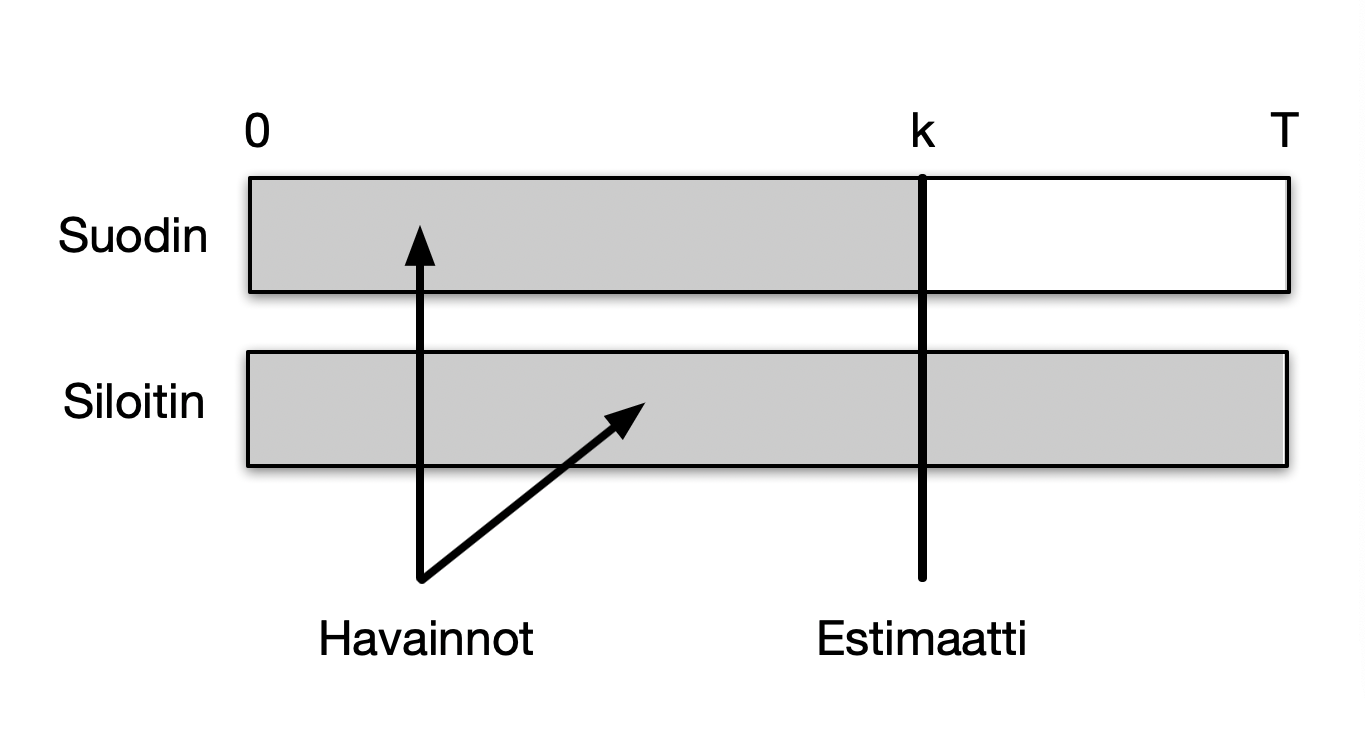
\includegraphics[width=9cm]{suodin_vs_siloitin_cropped}
\caption{Suodin- ja siloitteluongelma}
\label{fig:suodin_vs_siloitin}
\end{figure}

\section{Suodin- ja siloitteluongelmien historiaa}

Tämä alaluku esittää pääpiirteittään suodinongelmalle esitettyjen ratkaisujen historian. Lineaarisen suodinongelman osalta alaluku noudattaa Dan Crisanin artikkelia ``The stochastic filtering problem: a brief historical account'' (2014) \citep{crisan-2014} sekä Mohinder S. Grewalin ja Angus P. Andrewsin artikkelia ``Applications of Kalman Filtering in Aerospace 1960 to the Present'' (2010) \citep{Grewal-2010}. Hiukassuotimien osalta lähteenä toimii Cappé \&al (2007) \citep{cappe-2007}.

Suodinongelma nousi esille insinööritieteiden sekä sotateollisuuden käytännön ongelmista 2. maailmansodan aikana, vaikkakin suodinongelman diskreetin ajan ratkaisut juontavat jo Andrei N. Kolmogorovin 30-luvun artikkeleihin. Jatkuvan ajan tilanteessa ensimmäisen optimaalisen, kohinan sallivan suotimen esitti matemaatikko, kybernetiikan kehittäjä Norbert Wiener. Wiener-suotimena tunnettua ratkaisuaan varten Wiener muotoili seuraavat kolme ominaisuutta, jotka prosessin \(X\) estimaatin \(\hat{X}_t\) pitää toteuttaa.

\begin{enumerate}
\vspace{\baselineskip}
\item \textit{Kausaliteetti}: $X_t$ tulee estimoida käyttäen arvoja $Y_s$, missä $s \leq t$.
\item \textit{Optimaalisuus}: $X_t$:n estimaatin $\hat{X}_t$ tulee minimoida keskineliövirhe $\mathbb{E}[(X-\hat{X}_t)^2]$.
\item \textit{On-line -estimointi}: Estimaatin $\hat{X}_t$ tulee olla saatavissa minä hyvänsä ajanhetkenä $t$. 
\vspace{\baselineskip}
\end{enumerate}

Wiener sovelsi ratkaisussaan stationaaristen prosessien spektriteoriaa. Tulokset julkaistiin salaisina Yhdysvaltojen asevoimien tutkimuksesta vastanneen National Defense Research Committeen (NDRC) raportissa vuonna 1942. Tutkimus tunnettiin sodan aikana lempinimellä ``Keltainen vaara'' sekä painopaperinsa värin että vaikeaselkoisuutensa vuoksi. Myöhemmin Wiener esitti tuloksensa julkisesti kirjassaan \textit{Extrapolation, Interpolation and Smoothing of Stationary Time Series} (1949). Wienerin alkuperäiset kolme perusperiaatetta päteveät edelleen kaikille suodinongelman ratkaisuille, myös hiukassuotimille.

Kenties tärkein ja varmasti tunnetuin lineaariseen suodinongelman ratkaisu on Kalman-suodin. Suotimen kehittivät R.E. Kalman ja R.S. Bucy 1950- ja 60-lukujen taitteessa Yhdysvaltain kylmän sodan kilpavarustelutarpeisiin perustetussa Research Institute for Advanced Studies -tutkimuslaitoksessa (RIAS). Kalman-suodin on suodinongelman diskreetin ajan ratkaisu, kun taas Kalman-Bucy-suodin on jatkuvan ajan ratkaisu. Kohinan ollessa normaalijakautunutta on Kalman-suodin Wiener-suotimen tavoin lineaarisen suodinongelman optimaalinen ratkaisu. Wiener-suotimella ja Kalman-suotimella on kuitenkin erilaiset oletukset, minkä vuoksi erityisesti säätö- ja paikannussovelluksissa Kalman-suotimen käyttö on luontevampaa. Suotimien oletuksia ja oletusten välisiä eroja ei käsitellä tässä tutkielmassa, mutta alaluvussa 1.6. TODO:LINKKI käsitellään Kalman-suotimen formaalia yhteyttä hiukassuotimiin.

Kalman-suodinta voidaan soveltaa myös epälineaarisessa tapauksessa, kunhan suodinongelman funktiot \(f(\cdot)\) ja \(h(\cdot)\) ovat derivoituvia ja niihin liittyvä kohina oletetaan normaalijakautuneeksi. Tätä ratkaisua kutsutaan laajennetuksi Kalman-suotimeksi (extended Kalman filter, EKF). Suodin kehitettiin 60-luvulla NASA:n Apollo-ohjelman tarpeisiin, vaikkakin itse avaruusalusten laitteistot hyödynsivät lentoratojen laskennassa Kalman-suotimen perusversiota. Laajennetun Kalman-suotimen toimintaperiaate perustuu epälineaaristen funktioiden linearisointiin Taylorin kehitelmän avulla kulloisenkin estimaatin ympärillä. Laajennettu Kalman-suodin on erityisesti paikannussovellusten \textit{de facto} -suodinstandardi, mutta suodin ei kuitenkaan ole epälineaarisen ongelman optimaalinen estimaattori.

Kalman-suotimesta on lisäksi olemassa lukuisia muita epälineaarisiin ongelmiin soveltuvia laajennuksia, muun muassa paikkaratkaisun Kalman-suodin (\emph{position Kalman filter}, PKF), hajustamaton Kalman-suodin (\emph{unscented Kalman filter}, UKF) sekä tilastollisesti linearisoitu Kalman-suodin (\emph{statistically linearized Kalman filter}, SLF). Kuitenkin jos prosessin \(X\) mallia ei tunneta tarkasti tai kohinaa ei voida olettaa normaalijakautuneeksi, ovat hiukassuotimet eli sekventiaaliset Monte Carlo -menetelmät Kalman-suotimen johdannaisia parempia ratkaisuja. Vaikka tila-avaruuden dimensioiden kasvaessa kasvaa myös hiukassuotimien vaatima laskentateho, ovat hiukassuotimet aina sitä parempia mitä epälineaarisempia mallit ovat ja mitä kauempana normaalijakaumasta kohina on. Viimeisten vuosikymmenten aikana myös laskennan teho on kasvanut merkittävästi samalla kun laskennan hinta on vastaavasti romahtanut, mikä puoltaa Monte Carlo -menetelmien käyttöä entistä useammissa ongelmissa.

Joitakin suodinongelman rekursiivisia Monte Carlo -ratkaisuja löytyy jo 1950\textendash 70-luvuilta, erityisesti säätöteoriaan piiristä. Olennainen nykyalgoritmeihin periytynyt oivallus varhaisissa suodinalgoritmeissa oli tärkeytysotannan käyttö halutun jakaumaestimaatin laskennassa. Tärkeytysotanta-algoritmiin voidaan turvautua, kun emme pysty suoraan tekemään havaintoja jostakin jakaumasta \(p\) ja teemme sen sijaan havaintoja jakaumasta \(q\), jota painotamme niin, että tuloksena saadaan jakauman \(p\) harhaton estimaatti. Algoritmi on kuvattu tarkemmin tutkielman alaluvussa 2.

Tärkeytysotantaa käyttävä suodinongelman ratkaiseva SIS-algoritmi (\emph{sequential importance sampling}) ei kuitenkaan vielä 70-luvulla löytänyt suurta käytännön suosiota. Osin tämä johtui puutteellisesta laskentatehosta, mutta algoritmi kärsi myös otosten ehtymisenä (\emph{sample impoverishment}) tunnetusta ongelmasta. Monissa ongelmissa SIS-algoritmia käytettäessä suuri osa painoista päätyy vain tietyille partikkeleille, jolloin vastaavasti suuri osa partikkeleista ei enää estimoi haluttua jakaumaa. Tähän ongelmaan palataan myöhemmin.

Merkittävän ratkaisun ehtymisongelmaan esittivät Gordon, Salmond ja Smith artikkelissaan ``Novel approach to nonlinear/non-Gaussian Bayesian state estimation'' (1993). \citep{Gordon-1993} Artikkelin ratkaisu kulki nimellä \emph{bootstrap filter}, saapasremmisuodin. Saapasremmisuodin vältti ehtymisen uudellenotannalla, jossa matalapainoiset partikkelit korvattiin otoksilla korkeapainoisemmista partikkeleista. Ratkaisussa painot eivät myöskään riippuneet partikkelien aiemmista poluista vaan ainoastaan havaintojen uskottavuusfunktiosta. Vastaavaa ratkaisua käytetään tämän tutkielman uudemmassa SIR-algoritmissa (\emph{sampling importance resampling}), jossa myös uudelleenotantaan sovelletaan tärkeytysotantaa.

Sekventiaalisissa Monte Carlo -menetelmissä stokastisen prosessin posteriorijakauman esittämiseen käytettyjä otoksia kutsutaan myös partikkeleiksi ja menetelmiä siten hiukassuotimiksi. Erityisesti myöhemmin esitettävää SIR-algoritmia kutsutaan usein hiukkassuotimeksi. Termiä hiukkassuodin käytti ensimmäisen kerran Del Moral artikkelissa ``Nonlinear Filtering: Interacting Particle Resolution'' (1996) \citep{DelMoral-1996}, SMC-menetelmät termiä Liu ja Chen artikkelissa ``Sequential Monte Carlo Methods for Dynamic Systems'' (1998) \citep{Liu-1998}. Tässä tutkielmassa käytetään yleisemmin käytettyä termiä hiukassuotimet.

\section{Monte Carlo -menetelmistä}

Tässä alaluvussa kuvataan lyhyesti hiukassuotimissa käytettävien Monte Carlo -menetelmien perusperiaate todennäköisyysjakauman estimoinnissa. Lisäksi esitetään tärkeytysotanta-algoritmi (\emph{importance sampling}), jonka tarkoituksena on estimoida harhattomasti jakaumaa \(p(x|y_{1:k})\), josta emme voi suoraan tehdä otoksia, mutta jota voimme approksimoida toisella jakaumalla \(q\). Esitykset noudattavat Särkkää (2013) \citep{sarkka-2013}.

\subsection{Monte Carlo -approksimaatio}

Bayesilaisessa päättelyssä ollaan yleisesti kiinnostuttu laskemaan johonkin posterioritiheysjakaumaan \(p\) liittyvää odotusarvoa

\begin{align}
\mathbb{E}[g(x)|y_{1:k}]=\int g(x)p(x|y_{1:k})dx,
\end{align}

\noindent missä \(g\) on tila-avaruuden mielivaltainen funktio ja \(p(x|y_{1:t})\) on havaintoihin \(\{y_1,\ldots,y_k\}\) liittyvä \(x\):n posterioritiheysjakauma. Odotusarvo on laskettavissa suljetussa muodossa vain harvoissa tapauksissa, suodinongelman kohdalla silloin, kun kyseessä on lineaarinen ja Gaussinen malli. Odotusarvoa voidaan kuitenkin approksimoida niin sanoituilla Monte Carlo -menetelmillä. Menetelmien perusperiaate on tehdä riippumattomia otoksia estimoitavasta jakaumasta ja laskea haluttu odotusarvo otosten avulla. Jos tehdään \(N\) otosta jakaumasta \(x^i\sim p(x|y_{1:t})\), missä \(i=\{1,\ldots,N\}\) saadaan näiden otosten avulla laskettua odotusarvon estimaatti

\begin{align}
\mathbb{E}[g(x)|y_{1:k}]\simeq\frac{1}{N}\sum_{i=1}^N g(x^i).
\end{align}

Monte Carlo -estimaatti konvergoi keskeisen raja-arvolauseen nojalla ja sen estimointivirheen voidaan osoittaa olevan luokkaa \(O(\frac{1}{\sqrt{N}})\) riippumatta tilamuuttujan \(x\) dimensiosta. Hiukassuotimet hyödyntävät Monte Carlo -estimointia sekventiaalisesti, jolloin estimaatti lasketaan rekursiivisesti kullekin ajanhetkelle \(k=\{1,\ldots, t\}\). Tähän palataan luvuissa 3 ja 4.

\subsection{Tärkeytysotanta}

Tilanteessa, jossa Monte Carlo -otoksia ei voida tehdä suoraan jakaumasta \(p\), voidaan hyödyntää jakaumaa \(p\) approksimoivaa tärkeytys- tai ehdotusjakaumaa \(q(x|y_{1:k})\) sekä ns. tärkeytysotantaa. Oletetaan, että tunnetaan priorijakauma \(p(x)\) ja on olemassa havaintomalli \(p(y_{1:k}|x)\) sekä valittu ehdotusjakauma \(q(x|y_{1:k})\), josta voidaan tehdä otoksia. Ehdotusjakaumalta edellytetään lisäksi, että sen kantaja on suurempi tai yhtä suuri kuin jakauman \(p(x|y_{1:k})\) ja että se saa nollasta poikkeavia arvoja kaikkialla missä \(p(x|y_{1:k})\) saa nollasta poikkeavia arvoja. Kirjoitetaan halutun posteriorijakauman odotusarvo integraalina

\begin{align}
\int g(x)p(x|y_{1:k})dx=\int g(x)\frac{p(x|y_{1:k})}{q(x|y_{1:k})}q(x|y_{1:k})dx,
\end{align}

\noindent jolle voidaan muodostaa Monte Carlo -approksimaatio tekemällä \(N\) otosta jakaumasta \(x^i \sim q(x|y_{1:k})\).

Muodostetaan näin odotusarvo

\begin{align}
\mathbb{E}[g(x)|y_{1:k}]\simeq\frac{1}{N}\sum_{i=1}^N\frac{p(x^i|y_{1:k})}{q(x^i|y_{1:k})}g(x^i)=\sum_{i=1}^Nw^ig(x^i),
\end{align}

\noindent missä \(g(x)\) on jokin estimoinnissa hyödyllinen, mielivaltainen funktio. Tutkielmassa käytetty notaatio \(x_k^i\) viittaa ajanhetken \(k\) partikkeliin \(i\), missä \(i=\{1,\ldots,N\}\). Tärkeytysotantaa kuvaa nyt algoritmi (\ref{tarkeytysotanta-algo}). Kun posteriorijakauman estimaatti muodostetaan kyseisellä algoritmilla voidaan tulos kirjoittaa

\begin{align}
\hat{p}(x|y_{1:k})=\sum_{i=1}^{N}w^i \delta(x-x^i),
\end{align}

\noindent missä \(\delta(x)\) on Diracin deltafunktio.

\begin{algorithm}[H]
\label{tarkeytysotanta-algo}
\DontPrintSemicolon
\Begin{
  \For{$i=1,2,\ldots,N$}{
    \Begin{Otetaan $N$ otosta ehdotusjakaumasta $x^i \sim q(x|y_{1:k}).$}
    \Begin{Lasketaan normalisoimattomat painot $w_*^i= p(y_{1:k}|x^i)p(x^i)/q(x^i|y_{1:k}).$ \newline ja normalisoidut painot $w^i=w_*^i/\sum_{j=1}^Nw_*^j$.}
    \Begin{Estimoidaan $p$ laskemalla tiheydelle approksimaatio $\mathbb{E}[g(x)|y_{1:k}]\simeq\sum_{i=1}^Nw^ig(x^i)$.}
    } 
  }  
\caption{Tärkeytysotanta}
\end{algorithm}

\section{Bayesilainen suodin}

Suodinongelmassa ollaan kiinnostuttu tilavektorin posteriorijakauman \(p(x_k|y_{1:k})\) estimoinnista. Tässä alaluvussa käydään läpi yleinen rekursiivinen, Bayesilainen posteriorijakauman laskenta. Tällaista suodinongelman ratkaisua kutsutaan myös Bayesilaiseksi suotimeksi. Koska epälineaarisessa, ei-normaalijakautuneessa tilanteessa rekursiota ei voida laskea analyyttisesti, pitää estimoinnissa käyttää numeerisia menetelmiä. SMC-menetelmissä tämä tarkoittaa jakauman sekventiaalista Monte Carlo -approksimointia, jonka toteutus esitetään alaluvun 4 algoritmissa. Molemmat esitykset noudattavat Gustafssonia (2010).

Bayesilainen ratkaisu tilavektorin posteriorijakauman estimaatille \(\hat{p}(x_k|y_{1:k})\) saadaan seuraavalla rekursiolla (käydään läpi jokaiselle ajanhetkelle \(k=\{1,\ldots,t\}\)). Lasketaan ensin

\begin{align}\label{bayes-paivitys}
p(x_k|y_{1:k}) = \frac{p(y_k|x_k)p(x_k|y_{1:k-1})}{p(y_k|y_{1:k-1})},
\end{align}

\noindent joka saadaan suoraan Bayesin kaavasta \(P(A|B)=P(B|A)P(A)/P(B)\). Normalisointivakio lasketaan integraalina

\begin{align}\label{bayes-normalisointi}
p(y_k|y_{1:k-1})=\int_{\mathbb{R}^{n_x}}p(y_k|x_k)p(x_k|y_{1:k-1})\mathop{dx_k},
\end{align}

\noindent joka saadaan kokonaistodennäköisyyskaavasta \(P(A)=\mathbb{E}[P(A|X)]=\int_{-\infty}^{\infty}P(A|X=x)f_X(x)\mathop{dx}\). Merkintä \({R}^{n_x}\) vastaa tässä piilossa olevan tilavektorin dimensiota \(n\).

Lopuksi lasketaan päivitysaskel ajalle, joka saadaan edelleen kokonaistodennäköisyydellä

\begin{align}\label{bayes-aikapaivitys}
p(x_{k+1}|y_{1:k})=\int_{\mathbb{R}^{n_x}}p(x_{k+1}|x_k)p(x_k|y_{1:k})\mathop{dx_k}.
\end{align}

\noindent Rekursion avulla voimme laskea jakauman \(p(x_k|y_{1:k})\) estimaatti käymällä rekursion läpi \(k\) kertaa.

\section{Kalman-suotimen ja hiukassuotimen yhteydestä ja eroista}

Tässä alaluvussa käsitellään lyhyesti Kalman-suotimen yhteyttä hiukassuotimeen edellä estitetyn teorian valossa. Esitys noudattaa Särkkää (2013). \citep{sarkka-2013} Merkitään kuten edellä dynaamista mallia \(x_k\) ja havaintomallia \(y_k\) ja oletataan toisin kuin edellä, että nämä ovat lineaarisia ja noudattavat normaalijakaumaa. Koska mallit ovat lineaarisia, voidaan ne nyt kirjoittaa muotoon

\begin{align}
&\label{kalman-malli1}x_k=\mathbf{A}_{k-1}x_{k-1}+q_{k-1},\\
&\label{kalman-malli2}y_k=\mathbf{H}_k x_k + r_k
\end{align}

missä \(\mathbf{A}_{k-1}\) on dynaamisen mallin tilasiirtymään kuvaava matriisi ja \(\mathbf{H}_k\) on havaintojen mallimatriisi. Normaalisuusoletuksesta puolestaan seuraa, että sekä mallin että prosessin kohinavektorit noudattavat normaalijakaumia \(q_{k-1} \sim \mathbb{N}(0, \mathbf{Q}_{k-1})\) ja \(r_k \sim \mathbb{N}(0, \mathbf{R}_k)\), missä \(\mathbf{Q}_{k-1}\) ja \(\mathbf{R}_k\) ovat kovarianssimatrsiiseja. Lisäksi oletetaan, että prosessin priorijakauma on normaali eli \(x_0 \sim \mathbb{N}(m_0, \mathbf{P_0})\). Mallit voidaan nyt kirjoittaa tiheysfunktiomuodossa

\begin{align}
&\label{kalman-malli-pdf1}p(x_k|x_{k-1})=\mathbb{N}(x_k|\mathbf{A}_{k-1}x_{k-1},\mathbf{Q}_{k-1})\\
&\label{kalman-malli-pdf2}p(y_k|x_k)=\mathbb{N}(y_k|\mathbf{H}_{k}x_{k},\mathbf{R}_{k})
\end{align},

joista voidaan edelleen johtaa suodinongelman mallit

\begin{align}
&\label{kalman-malli-suodin1}p(x_k|y_{1:k-1})=\mathbb{N}(x_k|m_k^* ,\mathbf{P}_k^*)\\
&\label{kalman-malli-suodin2}p(x_k|y_{1:k})=\mathbb{N}(x_k|m_k ,\mathbf{P}_k)\\
&\label{kalman-malli-suodin3}p(y_k|y_{1:k-1})=\mathbb{N}(y_k|\mathbf{H}_k m_k^* ,\mathbf{S}_k)
\end{align}

ja ongelma ratkaista näin algoritmilla \(\ref{kf}\).

\begin{algorithm}[H]
\label{kf}
\DontPrintSemicolon
\SetAlgoShortEnd
\KwResult{Posteriorijakauman $p(x_{1:k}|y_{1:k})$ estimaatti.\;}
\KwData{Havainnot $y_k$. Priorijakauman $x_0$ keskiarvovektori $m_0$ ja kovarianssimatriisi $P_0$.\;}
\Begin{
  \For{$k=\{1,2,\ldots,t\}$}{
    \Begin{Ennusteaskel. \newline $m_k^*= \mathbf{A}_{k-1}m_{k-1}$\;}
    \If{$k < t$}{\Begin{Päivitysaskel. \newline $v_k = y_k - \mathbf{H}_k m_k^*$
    \newline $\mathbf{S}_k = \mathbf{H}_k \mathbf{P}_k^* \mathbf{H}_k^\top + \mathbf{R}_k$
    \newline\ $\mathbf{K}_k = \mathbf{P}_k^* \mathbf{H}_k^\top \mathbf{S}_k^{-1}$
    \newline\ $m_k = m_k^* \mathbf{K}_k v_k$
    \newline\ $\mathbf{P}_k = \mathbf{P}_k^* - \mathbf{K}_k \mathbf{S}_k \mathbf{K}_k^\top$;}}
  }  
}
\caption{Kalman-suodin}
\end{algorithm}

Esitetty algoritmi on ns. Kalman-suodin, joka selkeästi toimii suodinongelman ratkaisuna, kun mallit ovat haluttua lineaarista normaalimuotoa. Jos tämä oletus ei täyty, on Kalman-suotimesta kehitetty useita versioita, joissa ei-lineaarinen malli voidaan linearisoida tiettyjen ehtojen vallitessa. Tämän lyhyen alaluvun tarkoituksena oli esittää, että Kalman-suotimessa ongelma on samaa muotoa kuin hiukassuotimessa, joten linearisoituja Kalman-suotimia ei tässä käsitellä. Hiukassuodin myös ratkaisee ongelman mille hyvänsä epälineaariselle mallille.

\chapter{Hiukassuotimet}

\section{SIR-algoritmi}

Tässä alaluvussa esitetään SMC-menetelmiin kuuluva SIR-algoritmi, epälineaarisen suodinongelman ratkaisemiseksi. Algoritmi on numeerinen toteutus alaluvussa 3 kuvatusta Bayesilaisesta suotimesta. Esitetty algoritmi perustuu Gustafssoniin (2010). Ilman uudelleenotantavaihetta kyseessä olisi SIS-algoritmi.

Algoritmi alustetaan jakaumasta \(x_1^i\sim p_{x_0}\) generoiduilla \(N\)-kappaleella partikkeleita. Jokaiselle partikkelille annetaan alustuksessa sama paino \(w_{1|0}^i=1/N\). Algoritmi suoritetaan jokaiselle partikkelille \(i=\{1,2,\ldots,N\}\) jokaisella ajanhetkellä \(k=\{1,2,\ldots,t\}\).

Seuraava toistetaan jokaiselle ajanhetkelle \(k=\{1,2,\ldots,t\}\). Algoritmin ensimmäisessä vaiheessa päivitetään painot yhtälön (\ref{painopaivitys}) mukaan.

\begin{align}\label{painopaivitys}
w^i_{k|k}=\frac{1}{c_k}w^i_{k|k-1}p(y_k|x^i_k).
\end{align}

\noindent Tämä vastaa yllä esitetyn Bayes-suotimen päivitysvaihetta (\ref{bayes-paivitys}). Normalisointipaino \(c_k\) lasketaan puolestaan yhtälöstä (\ref{normalisointi}), mikä vastaa Bayes-suotimen normalisointivakion laskemista (\ref{bayes-normalisointi}) ja asettaa painojen summaksi \(\sum_{i=1}^Nw^i_{k|k}=1\).

\begin{align}\label{normalisointi}
c_k=\sum_{i=1}^{N}w_{k|{k-1}}^ip(y_k|x_k^i).
\end{align}

\noindent Seuraavassa vaiheessa estimoidaan \(p\) laskemalla tiheyden \(p(x_{1:k}|y_{1:k})\) Monte Carlo -estimaatti yhtälön (\ref{p-estimaatti}) perusteella

\begin{align}\label{p-estimaatti}
\hat{p}(x_{1:k}|y_{1:k})=\sum_{i=1}^{N}w_{k|k}^i \delta(x_{1:k}-x_{1:k}^i).
\end{align}

Tämän jälkeen suoritetaan valinnainen uudelleenotanta. Uudelleenotanta voidaan tehdä jokaisella askeleella tai efektiivisen otoskoon perusteella alla kuvatun kynnysarvoehdon \(\hat{N}_{eff}< N_{th}\) täyttessä, jolloin uudelleenotantaa kutsutaan adaptiiviseksi uudelleenotannaksi. Tällaista uudelleenotantaa hyödynnetään esitetyssä algoritmissa (\ref{sir}) . Uudelleenotantaa tarkastellaan lähemmin alaluvussa 4.1.2.
Lopuksi päivitetään aika (jos \(k < t\)), luodaan uudet ennusteet partikkeleille ehdotusjakaumasta (\ref{ehdotusjakauma})

\begin{align}\label{ehdotusjakauma}
x_{k+1}^i\sim q(x_{k+1}|x_k^i,y_{k+1})
\end{align}

\noindent ja päivitetään partikkelien painot tärkeytysotannalla (\ref{tarkeytys}), sen mukaan kuinka todennäköisiä partikkelien ennusteet ovat

\begin{align}\label{tarkeytys} w_{k+1|k}^i=w_{k|k}^i\frac{p(x_{k+1}^i|x_k^i)}{q(x_{k+1}^i|x_k^i,y_{k+1})}.
\end{align}

\noindent Vaiheet \ref{ehdotusjakauma} ja \ref{tarkeytys} vastaavat Bayes-suotimen aikapäivitystä (\ref{bayes-aikapaivitys}).

Alla käsitellään algoritmiin liittyvän uudelleenotantamenetelmän, partikkelien määrän ja ehdotusjakauman valinta. Lopuksi esiteetään algoritmin konvergenssia, marginaalijakaumaa sekä aikakompleksisuutta koskevia tuloksia.

\begin{algorithm}[H]
\label{sir}
\DontPrintSemicolon
\SetAlgoShortEnd
\KwResult{Posteriorijakauman $p(x_{1:k}|y_{1:k})$ estimaatti.\;}
\KwData{Havainnot $y_k$. Generoitu $x_1^i\sim p_{x_0}$ missä $i=\{1,\ldots,N\}$ ja jokainen partikkeli saa saman painon $w_{1|0}^i=1/N$.\;}
\Begin{
  \For{$k=\{1,2,\ldots,t\}$}{
    \For{$i=\{1,2,\ldots,N\}$}{
      \Begin{Päivitetään painot $w_{k|k}.$\;}
      \Begin{Estimoidaan $p$ laskemalla tiheydelle approksimaatio $\hat{p}(x_{1:k}|y_{1:k})=\sum_{i=1}^{N}w_{k|k}^i \delta(x_{1:k}-x_{1:k}^i)$.\;}
    }
    \Begin{Lasketaan efektiivinen otoskoko $\hat{N}_{eff}$.\;}
    \If{$\hat{N}_{eff}< N_{th}$}{\Begin{Otetaan uudet $N$ otosta palauttaen joukosta $\{x_{1:k}^i\}_{i=1}^N$, missä otoksen $i$ todennäköisyys on $w^i_{k|k}$.\;}
    \Begin{Asetetaan painot $w^i_{k|k}=1/N$.\;}}
    \If{$k < t$}{\Begin{Aikapäivitys. \newline Luodaan ennusteet partikkeleille ehdotusjakaumasta $x_{k+1}^i\sim q(x_{k+1}|x_k^i,y_{k+1})$, \newline päivitetään partikkelien painot tärkeytysotannalla.\;}}
  }  
}
\caption{SIR}
\end{algorithm}

\subsection{Parametrien valinta}

Ennen algoritmin suorittamista valitaan ehdotusjakauma \(q(x_{k+1}|x_{1:k},y_{k+1})\), uudelleenotantamenetelmä sekä partikkelien määrä \(N\). Ehdotusjakauman ja uudelleenotantamenetelmän valinnassa tärkeimpänä päämääränä on välttää otosten ehtymistä, kun taas partikkelien määrä säätelee kompromissia algoritmin suorituskyvyn ja tarkkuuden välillä.

\subsubsection{Otoskoon $N$ valinta}

Yleispätevää sääntöä otoskoon/partikkelien lukumäärän \(N\) valinnalle on vaikeaa antaa, sillä vaadittava estimointitarkkuus riippuu usein käsillä olevasta ongelmasta. Gordon \&al.~(1993) esittävät kuitenkin kolme tekijää, jotka vaikuttavat partikkelien lukumäärän valintaan

\begin{enumerate}
\def\labelenumi{\alph{enumi}.}
\tightlist
\item
  tila-avaruuden ulottuvuuksien lukumäärä \({n_x}\),
\item
  tyypillinen päällekäisyys priorin ja uskottavuuden välillä
\item
  sekä tarvittava aika-askelten lukumäärä.
\end{enumerate}

Ensimmäisen tekijän vaikutus on selvä. Mitä useammassa ulottuvuudessa otantaa tarvitsee tehdä, sen korkeammaksi on \(N\) asetettava, jotta jokainen ulottuvuus pystytään kattamaan. Tekijät (\textit{b}) ja (\textit{c}) puolestaan seuraavat uudelleenotannasta. Jos se osa tila-avaruutta, jossa uskottavuus \(p(y_k|x_k)\) saa merkittäviä arvoja on pieni verrattuna siihen osaan, jossa priorijakauma \(p(x_k|y_{1:k-1})\) saa merkittäviä arvoja, suuri osa partikkeleista saa pieniä painoja eikä näin valikoidu uudelleenotantaan.

Yleisesti ottaen \(N\) kannattaa asettaa sellaiseksi, että se paitsi tuottaa riittävän tarkan estimaatin, on se käytettävissä olevan laskentatehon sekä vaadittavan laskentanopeuden kannalta järkevää. Tähän palataan tutkielman lopuksi empiirisessä paikannusesimerkissä.

\subsubsection{Uudelleenotantamenetelmän valinta}

Ilman uudelleenotantaa on mahdollista, että algoritmi alkaa kärsiä SIS-algoritmille ominaisesta otosten ehtymisestä. Toisin sanoen kaikki painot alkavat keskittyä vain muutamalle partikkelille eikä algoritmi enää approksimoi tehokkaasti haluttua jakaumaa. Uudelleenotanta tarjoaa osittaisen ratkaisun tähän ongelmaan, mutta hävittää samalla informaatiota ja siten lisää satunnaisotantaan liittyvää epävarmuutta. Yleisesti ottaen uudelleenotanta kannattaa aloittaa vasta siinä vaiheessa algoritmin suorittamista, kun siitä on otosten ehtymisen kannalta hyötyä, esimerkiksi efektiivisen otoskoon pudottua jonkin kynnysarvon alapuolelle (adaptiivinen uudelleenotanta). Efektiivinen otoskoko saadaan laskettua variaatiokertoimesta \(c_\nu\) kaavalla

\begin{align}\label{N-eff}
N_{eff}= \frac{N}{1+c_\nu^2(w^i_{k|k})} = \frac{N}{1+\frac{\text{Var}(w^i_{k|k})}{(\mathbb{E}[w^i_{k|k}])^2}} =\frac{N}{1+N^2\text{Var}(w^i_{k|k})}.
\end{align}

Näin laskettu efektiivinen otoskoko maksimoituu (\(N_{eff}=N\)), kun kaikille painoille pätee \(w^i_{k|k}=1/N\) ja minimoituu (\(N_{eff}=1\)), kun \(w^i_{k|k}=1\) todennäköisyydellä \(1/N\) ja \(w^i_{k|k}=0\) todennäköisyydellä \((N-1)/N\). Normalisoitujen painojen avulla saadaan effektiiviselle otoskoolle ajanhetkellä \(k\) laskennallinen approksimaatio

\begin{align}\label{N-hat-eff}
\hat{N}_{eff}=\frac{1}{\sum_{i=1}^N(w^i_{k|k})^2}.
\end{align}

Sekä määritelmälle (\(\ref{N-eff}\)) että (\(\ref{N-hat-eff}\)) pätee \(1 \leq \hat{N}_{eff} \leq N\). Yläraja saavutetaan, kun jokaisen partikkelin paino on sama. Alarajalle päädytään, kun kaikki paino keskittyy yksittäiselle partikkelille. Tästä saadaan määriteltyä algoritmille SIR-uudelleenotantaehto \(\hat{N}_{eff}< N_{th}\). Gustafsson (2010) esittää uudelleenotannan kynnysarvoksi esimerkiksi \(\hat{N}_{th}=2N/3\).

Uudelleenotanta ei muuta approksimoitavan jakauma \(p\) odotusarvoa, mutta se lisää jakauman Monte Carlo -varianssia. On kuitenkin olemassa esimerkiksi osittamiseen perustuvia uudelleenotantamenetelmiä, jotka pyrkivät minimoimaan varianssin lisäyksen. Varianssin pienennysmenetelmät jätetään tämän tutkielman ulkopuolelle.

\subsubsection{Ehdotusjakauman valinta}

Yksinkertaisin muoto ehdotusjakaumalle on \(q(x_{1:k}|y_{1:k})\) eli jokaisella algoritmin suorituskerralla käydään läpi koko aikapolku \(1:k\). Tämä ei kuitenkaan ole tarkoituksenmukaista, erityisesti jos kyseessä on reaaliaikainen sovellutus. Kirjoitetaan ehdotusjakauma muodossa

\begin{align}\label{proposal-factorization}
q(x_{1:k}|y_{1:k})=q(x_k|x_{1:k-1},y_{1:k})q(x_{1:k-1}|y_{1:k}).
\end{align}

Jos yhtälöstä (\ref{proposal-factorization}) poimitaan ehdotusjakaumaksi ainoastaan termi \(q(x_k|x_{1:k-1},y_{1:k})\) voidaan tämä kirjoittaa edelleen Markov-ominaisuuden nojalla muotoon \(q(x_k|x_{k-1},y_{k})\). Tämä on suodinongelman kannalta riittävää, koska olemme kiinnostuneita posteriorijakaumasta ja arvosta \(x\) ainoastaan ajanhetkellä \(k\) (tasoitusongelmassa tarvitsisimme koko polun \(x_{1:k}\)). Alla tarkastellaan edelleen Gustafssonia (2010) seuraten kahta ehdotusjakauman valintatapaa, prioriotantaa (prior sampling) sekä uskottavuusotantaa (likelihood sampling).

Ennen ehdotusjakauman tarkastelua määritellään mallille signaali-kohinasuhde uskottavuuden maksimin ja priorin maksimin välisenä suhteena

\begin{align}\label{SNR}
\text{SNR}\propto \frac{\text{max}_{x_k}p(y_k|x_k)}{\text{max}_{x_k}p(x_k|x_{k-1})}. 
\end{align}

\noindent Yhdistetään lisäksi ehdotusjakaumia varten yhtälöt (\ref{painopaivitys}) ja (\ref{normalisointi}), jolloin saadaan painojen päivitys muotoon

\begin{align}\label{painopaivitys-propto}
w^i_{k|k} \propto w^i_{k-1|k-1}\frac{p(y_k|x^i_k)p(x_k|x^{k-1})}{q(x_k|x^i_{k-1},y_k)}.
\end{align}

Kun suhde (\ref{SNR}) on matala, on prioriotanta luonnollinen valinta. Tässä käytetään ehdotusjakaumana tilavektorin ehdollista prioria eli

\begin{align}\label{prioriotanta-q}
q(x_k|x_{1:k-1},y_{k})=p(x_k|x^i_{k-1}).
\end{align}

\noindent Yhtälön (\ref{prioriotanta-q}) perusteella saadaan edelleen prioriotannan painoiksi

\begin{align}\label{prioriotanta-w}
w^i_{k|k} = w^i_{k|k-1}p(y_k|x^i_k) = w^i_{k-1|k-1}p(y_k|x^i_k).
\end{align}

Kun signaali-kohinasuhde on kohtalainen tai korkea, on parempi käyttää ehdotusjakaumana skaalattua uskottavuusfunktiota (\ref{uskottavuusotanta-q}). Tarkastellaan ensin tekijöihin jakoa

\begin{align}\label{uskottavuusotanta-factorization}
p(x_k|x^i_{k-1},y_k)=p(y_k|x_k)\frac{p(x_k|x^i_{k-1})}{p(y_k|x^i_{k-1})}.
\end{align}

\noindent Kun SNR on korkea ja uskottavuusfunktio on integroituva pätee \(p(x_k|x^i_{k-1},y_{k}) \propto p(y_k|x_k)\), jolloin voidaan asettaa (\ref{uskottavuusotanta-q})

\begin{align}\label{uskottavuusotanta-q}
q(x_k|x^i_{k-1},y_{k}) \propto p(y_k|x_k).
\end{align}

\noindent Yhtälön (\ref{uskottavuusotanta-q}) perusteella saadaan edelleen uskottavuusotannan painoiksi (\ref{uskottavuusotanta-w}).

\begin{align}\label{uskottavuusotanta-w}
w^i_{k|k} = w^i_{k-1|k-1}p(x^i_k|x^i_{k-1}).
\end{align}

\subsection{Konvergenssituloksia}

Alla esitetään kaksi SIR-algoritmiin liittyvää konvergenssitulosta. Se, kuinka hyvin esitetyllä algoritmilla arvioitu posterioritiheys \(\hat{p}(x_{1:k}|y_{1:k})\) approksimoi todellista tiheysfunktiota \(p(x_{1:k}|y_{1:k})\) sekä mikä on approksimaation keskineliövirhe. Tulokset 1\textendash 2 noudattavat Crisanin ja Doucet'n artikkeleita ``Convergence of Sequential Monte Carlo Methods'' (2000) \citep{crisan-2000} ja ``A Survey of Convergence Results on Particle Filtering Methods for Practitioners'' (2002) \citep{crisan-2002}, tulos 3 Chopinin artikkelia ``Central limit theorem for sequential Monte Carlo methods and its application to Bayesian inference'' (2004) \citep{chopin-2004}.

\textit{Konvergenssitulos 1}: Kun \(N \to \infty\) algoritmille pätee \(\forall k\) tulos (\ref{jakaumakonvergenssi}).

\begin{align}\label{jakaumakonvergenssi}
\hat{p}(x_{1:k}|y_{1:k}) \xrightarrow{a.s.} p(x_{1:k}|y_{1:k}).
\end{align}

\textit{Konvergenssitulos 2}: Keskineliövirheelle pätee asymptoottinen konvergenssi (\ref{MSE-konvergenssi}).

\begin{align}\label{MSE-konvergenssi}
\mathbb{E}(\hat{g}(x_k)-\mathbb{E}(g(x_k)))^2\leq\frac{p_k\norm{g(x_k)}}{N},
\end{align}

\noindent missä \(g\) on mikä hyvänsä piilossa olevan tila-avaruuden rajoitettu Borel-mitallinen funktio (\(g \in \mathcal{B}(\mathbb{R}^{n_x})\)), \(\norm{g(\cdot)}\) kyseisen funktion supremum-normi ja \(p_k\) jokin äärellinen vakio, jolle pätee ajanhetkestä \(k\) riippumatta \(p_k=p<\infty\).

\textit{Konvergenssitulos 3}: Keskeinen raja-arvolause (\ref{CLT}).

\begin{align}\label{CLT}
\text{Kun } N \to \infty: \sqrt{N} \left\{ \frac{1}{N} \sum_{i=1}^N \hat{g}(x_k^i) -\mathbb{E}(g(x_k^i)) \right\} \xrightarrow{D} \mathbb{N}(0,\sigma^2 < \infty),
\end{align},

missä \(g\) on jälleen mikä hyvänsä piilossa olevan tila-avaruuden rajoitettu Borel-mitallinen funktio (\(g \in \mathcal{B}(\mathbb{R}^{n_x})\)). Konvergenssituloksia ei tämän tutkielman puitteissa todisteta.

\subsection{Marginaalijakauma}

Edellä kuvattu algoritmi 1 tuottaa approksimaation koko prosessin posteriorijakaumalle \(p(x_{1:k}|y_{1:k})\). Jos halutaan tietää ainoastaan posteriorijakauman \(p(x_k|y_{1:k})\) estimaatti, voidaan käyttää yksinkertaisesti viimeisestä tilasta \(x_k\) laskettua estimaattia

\begin{align}
\hat{p}(x_{k}|y_{1:k})=\sum_{i=1}^{N}w_{k|k}^i \delta(x_{k}-x_{k}^i).
\end{align}

Toinen, tarkempi vaihtoehto on käyttää laskennassa tärkeytyspainoa

\begin{align}\label{marginaalitarkeytys}
w_{k+1|k}^i=\frac{\sum_{j=1}^{N}w_{k|k}^jp(x_{k+1}^i|x_k^j)}{q(x_{k+1}^i|x_k^i,y_{k+1})}
\end{align}

\noindent painon (\ref{tarkeytys}) sijaan. Tällöin jokaisella aikapäivitysaskeleella lasketaan painot kaikkien mahdollisten tila-aika-avaruuspolkujen yli. Samoin kuin uudelleenotanta tämä pienentää painojen varianssia.

\subsection{Aikakompleksisuus}

Algoritmin perusmuodon aikakompleksisuus on \(\mathcal{O}(N)\). Uudelleenotantamenetelmän tai ehdotusjakauman valinta ei suoraan vaikuta aikakompleksisuuteen. Sen sijaan marginalisointi tärkeytyspainolla (\ref{marginaalitarkeytys}) lisää algoritmin aikakompleksisuutta \(\mathcal{O}(N)\rightarrow\mathcal{O}(N^2)\), koska jokaisen partikkelin kohdalla painot lasketaan jokaisen tila-aika-avaruuspolun yli. On selvää, että erityisesti isoilla otoskoon \(N\) arvoilla ei yllä esitetty marginalisointi enää ole mielekästä.

Tällaisia tilanteita varten algoritmista on olemassa \(\mathcal{O}(N\text{log}(N))\) -versioita, jotka perustuvat esimerkiksi N:n kappaleen oppimiseen (N-body learning). Näiden algoritmien käsittely jää tämän tutkielman ulkopuolelle, mutta katsauksen algoritmeista ovat esittäneet esimerkiksi Klaas \&al.~artikkelissa ``Toward Practical \(N^2\) Monte Carlo: the Marginal Particle Filter'' (2012).

\section{Saapasremmisuodin}

Saapasremmisuodin \ref{saapasremmisuodin} eli \emph{bootsrtrap filter} on SIR-algoritmin muunnelma, jossa tärkeytysotannan (kts. \ref{tarkeytysotanta-algo}) käytetään dynaamista mallia \(p(x_k|x_{k-1})\).

\begin{algorithm}[H]
\label{saapasremmisuodin}
\DontPrintSemicolon
\SetAlgoShortEnd
\KwResult{Posteriorijakauman $p(x_{1:k}|y_{1:k})$ estimaatti.\;}
\KwData{Havainnot $y_k$. Generoitu $x_1^i\sim p_{x_0}$ missä $i=\{1,\ldots,N\}$ ja jokainen partikkeli saa saman painon $w_{1|0}^i=1/N$.\;}
\Begin{
  \For{$k=\{1,2,\ldots,t\}$}{
    \For{$i=\{1,2,\ldots,N\}$}{
      \Begin{Luodaan uudet estimaatit dynaamisesta mallista $x_{k}^i\sim p(x_{k}|x_{k-1}^i)$.;}
      \Begin{Päivitetään hiukkasten painot $w_k^i$ uskottavuusfunktion $p(y_k|x_k^i)$ mukaan.}
      \Begin{Estimoidaan $p$ laskemalla tiheydelle approksimaatio $\hat{p}(x_{1:k}|y_{1:k})=\sum_{i=1}^{N}w_{k|k}^i \delta(x_{1:k}-x_{1:k}^i)$.}
    }
    \If{$k < t$}{\Begin{Aikapäivitys. Suoritetaan uudelleenotanta kuten SIR-algoritmissa \ref{sir}.\;}}
  }  
}
\caption{Saapasremmisuodin}
\end{algorithm}

Saapasremmisuodin on edellä esitettyä SIR-algoritmia yksinkertaisempi toteuttaa, mutta epäinformatiivisen tärkeytysjakauman vuoksi algoritmi saattaa vaatia SIR-algoritmia suuremman määrän hiukkasia. Saapasremmisuodin esitetään tässä sen historiallisen tärkeyden vuoksi, sillä kyseessä oli ensimmäinen uudelleenotataantaa hyödyntävä hiukassuodinalgoritmi. Suotimen käytännön toteutukseen palataan luvussa 4.

\section{Varianssin estimoinnista}

Hiukassuotimen varianssin estimoinnissa ollaan kiinnostuneita jakaumaestimaatin \(\hat{p}(x_{1:k}|y_{1:k})\) varianssin estimoinnista. Yksinkertaisin tapa estimoida hiukassuodinalgoritmin varianssia on ajaa algoritmi \(M > 1\) kertaa. Koska ajot ovat toisistaan riippumattomia, voidaan estimaatin varianssi laskea kullekin ajanhetkelle \(k\) näiden ajojen \(k\)-hetken estimaattien otosvarianssina:

\begin{align}\label{MC-varianssi}
\hat{\sigma}^2_{MC} = \text{Var}_{\text{MC}}(\hat{p}(x_{1:k}|y_{1:k})) = \frac{1}{M-1} \sum_{i=1}^{M}(x_k^i-\bar{x_k})^2.
\end{align},

missä \(x_k^i\) on \(k\):nen ajanhetken piste-estimaatti ajolle \(i=1,\ldots,M\) ja \(\bar{x_k}\) piste-estimaattien aritmeettinen keskiarvo laskettuna kaikkien \(M\) ajojen yli. TODO: vektoroi. Tällaisen Monte Carlo -varianssin estimoiminen on kuitenkin laskennallisesti tehotonta. Monissa käytännön sovelluksissa jo yhden hiukassuodinalgoritmin ajaminen vaatii runsaasti laskentatehoa, jolloin Monte Carlo -varianssin laskeminen ei ole mahdollista. Varianssia ei voi myöskään laskea analyyttisesti, mutta koska keskeisen raja-arvolauseen \ref{CLT} nojalla tiedetään, että asymptoottinen varianssi

\begin{align}\label{asymptoottinen-varianssi}
\lim_{N\to \infty} N \text {Var}(\hat{g}(x_k^i))
\end{align},

on olemassa, on sen estimointiin on lähivuosina kehitetty joitakin menetelmiä. Alla käsitellään Leen ja Whitleyn (2018) ehdottamaa varianssin estimointitapaa. \citep{Lee-2018}

Ajetaan SIR-algoritmi kuten esitetty algoritmissa \ref{sir}, mutta merkitään kullakin algoritmin suorituskerralla \(k=1,\ldots,T\) ja jokaisella partikkelilla \(n=1,\ldots,N\) indeksillä \(E_k^n\) kunkin hiukkasen kantaisää eli toisin sanoen sitä hiukkasta, josta kyseinen hiukkanen on uudelleenotantojen kaltta polveutunut ajanhetkestä \(k=1\) lähtien. Kaavio \ref{fig:eeva-indeksit} havainnollistaa hiukkasten polveutumista.

\begin{figure}[H]
\centering
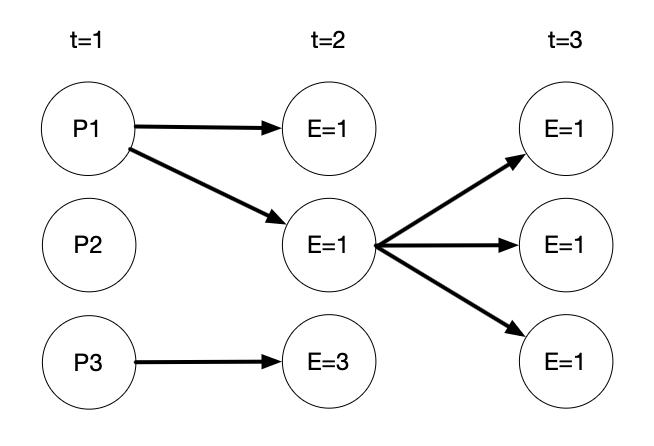
\includegraphics[width=9cm]{eevaindeksit}
\caption{Esimerkki Eeva-indekseistä, kun $T=3$ ja $N=3$.}
\label{fig:eeva-indeksit}
\end{figure}

Varianssiestimaatti voidaan laskea näiden, Leen ja Whitleyn Eeva-indekseiksi nimeämien indeksien perusteella seuraavasti:

\begin{align}\label{CLT-varianssi}
\hat{\sigma}^2_{CLT} = \frac{1}{N^2} \left[ (\sum_{i=1}^N \gamma(x_k^i))^2 - (\frac{N}{N-1})^{n+1} ( \sum_{i=1}^N \sum_{j:E_n^j=i} \gamma(x_k^i) \gamma(x_k^j)) \right]
\end{align},

missä \(\gamma: \mathbf{X}_n \rightarrow \mathbb{R}\) on rajoitettu, \(\mathcal{X}_n\)-mitallinen funktio. SIR-algoritmin kohdalla jakaumaestimaatti \(\hat{p}(x_{1:k}|y_{1:k}))\). Kyseessä on harhaton ja konsistentti asymptoottisen varianssin estimaatti. Tarkemmin \(N\hat{\sigma}^2_{CL}\) konvergoi asymptoottiseen varianssiin \ref{asymptoottinen-varianssi}. Tätä ei tutkielman puitteissa todisteta.

Yllä esitetty varianssiestimaatti kärsii kuitenkin epätarkkuudesta, sillä kun \(k \to \infty\) polveutuvat kaikki hiukkaset lopulta samasta kantaisästä eli indeksit \(E_k^i,\ldots,E_k^N\) ovat kaikki yhtäsuuria. Tämän vuoksi on mielekästä johtaa indeksit ainoastaan tietystä aiemmasta ajanhetkestä alkaen. Olsson ja Douc (2019) \citep{olsson-2019} ehdottavat tähän tarkoitukseen Henok-indeksiä \(E_{k,m}^n\), jossa \(m\) merkitsee ajanhetken \(m<k\) hiukkasta, josta kyseinen hiukkanen polveutuu. Hiukkasten kantaisien sukupolvi määritetään viipeellä \(\lambda\) niin, että \(m=k-\lambda\). Kaavio \ref{fig:henok-indeksit} havainnollistaa hiukkasten polveutumista, kun \(\lambda=1\).

\begin{figure}[H]
\centering
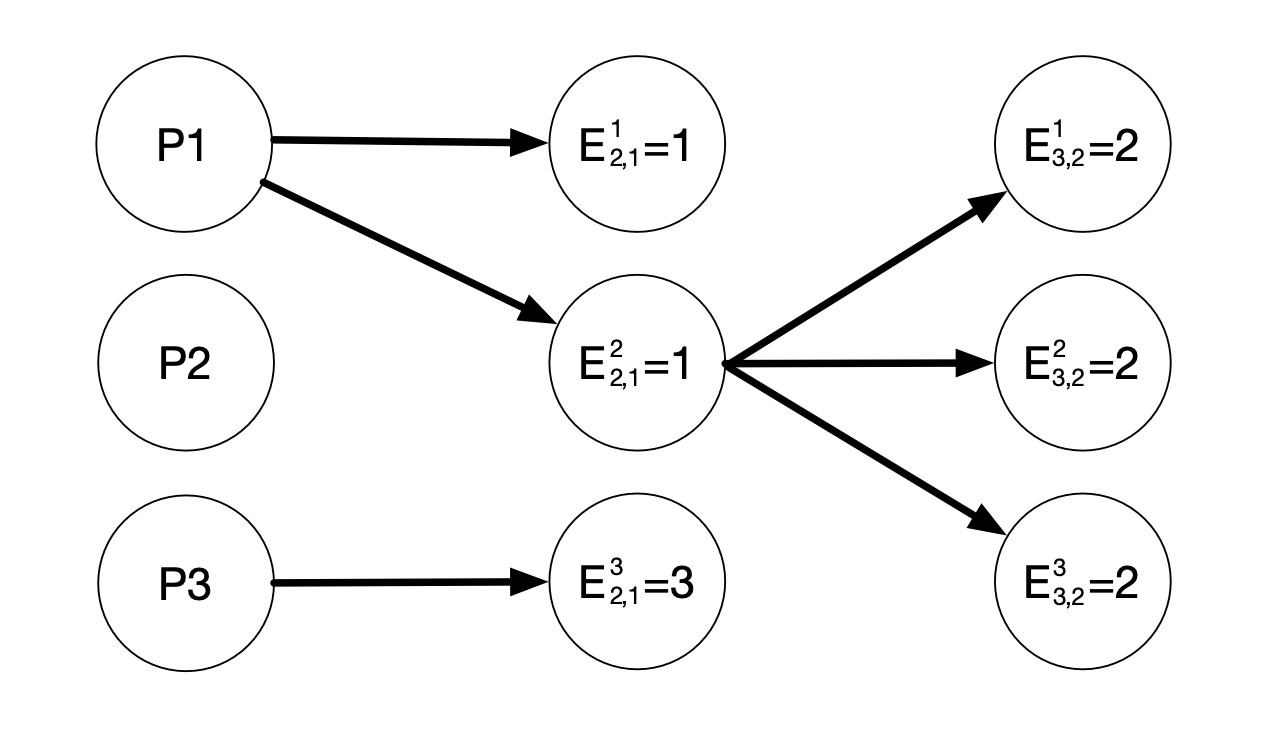
\includegraphics[width=9cm]{henokindeksit}
\caption{Esimerkki Henok-indekseistä, kun $T=3$, $N=3$ ja $\lambda=1$.}
\label{fig:henok-indeksit}
\end{figure}

Nyt varianssi saadaan muotoon

\begin{align}\label{OD-varianssi}
\hat{\sigma}^2_{OD} = \frac{1}{N^2} \left[ (\sum_{i=1}^N \gamma(x_k^i))^2 - (\frac{N}{N-1})^{n+1} ( \sum_{i=1}^N \sum_{j:E_{n,k(\lambda)}^j=i} \gamma(x_k^i) \gamma(x_k^j)) \right]
\end{align},

missä \(k(\lambda) \coloneq k-\lambda\). Viive \(\lambda\) on varianssiestimaatin suunnitteluparametri. Pienillä viipeillä estimaatti on harhainen, mutta harha laskee viipeen kasvaessa. Olsson ja Douc suosittavat viipeen ylärajaksi arvoa \(\lambda=20\), jolloin estimaattorin harha on käytännössä kokonaan hävitetty. Tämän jälkeen estimaatti voi myös alkaa kärsiä samasta epätarkkuudesta kuin Eeva-indekseihin perustuva CLT-estimaatti.

Mastrototaro ja Olsson (2023) \citep{Mastrototaro-2023} laajentavat tätä estimaattia edelleen niin, että viive \(\lambda\) valitaan mukautuvasti. Mastrototaron ja Olssonin ALvar-estimaatti (\emph{Adaptive-Lag variance}) lasketaan, kuten OD-varianssi edellä \ref{OD-varianssi}, mutta kunkin algoritmin ajokerran jälkeen asetetaan seuraavan ajanhetken \(\lambda\) seuraavasti:

\begin{align}\label{ALvar-lambda}
\lambda_{k+1} \leftarrow \operatorname*{arg\,max}_{\lambda \in [0, \lambda_k + 1]} \hat{\sigma}^2_{k+1,\lambda} (\gamma_{k+1})
\end{align},

Tämä perustuu havaintoon, jonka mukaan ehtyneille Henok-indekseille on olemassa \(\lambda^\prime \in [0, \lambda-1]\), joka täyttää ehdon \(\hat{\sigma}^2_{k+1,\lambda} (\gamma_{k+1}) < \hat{\sigma}^2_{k+1,\lambda^\prime} (\gamma_{k+1})\). Koska myös ehtyneiden indeksien kantaisät ovat ehtyneitä. Nyt indeksi \(\lambda_{n+1}\) voidaan valita rekursiivisesti niin, että se tuottaa suurimman varianssiestimaatin, joka on kuitenkin rajoitettu ylhäältä arvoon \(\lambda_n+1\). Tämä indeksi ei ole koskaan ehtynyt, joten se on myös parhaan varianssiestimaatin tuottava valinta.

Esitettyjä varianssiestimaatteja voidaan hyödyntää paitsi algoritmien ja parametrivalintojen vertailussa myös mukautuvan viipeen hiukassiloittimen viipeen valinnassa (kts. luku 4 LINKKI). Varianssiestimaattia hyödynnetään myös luvun 5 empiirisen esimerkin uskottavuusfunktioiden parametrien estimoinnissa.

\chapter{Hiukassilottimet}

Tässä luvussa käsitellään suodinongelmaan läheisesti liittyvän hiukassiloittimen ratkaisemista ns. hiukassiloitinalgoritmien avulla. Kuten hiukassuotimien kohdalla, myös tässä luvussa esitetään ongelma ensin yleisessä Bayesilaisessa muodossa, jonka jälkeen siirrytään käsittelemään hiukkasmenetelmiin pohjautuvia siloitinalgoritmeja. Luvussa käsiteltävät algoritmit jaetaan kahteen pääkategoriaan, offline-algoritmeihin, joita sovelletaan hiukassuodinalgoritmin ajon jälkeen sekä online-algoritmeihin, jotka suoritetaan yhdessä hiukassuodinalgoritmin kanssa. Siloitinongelman esittely seuraa Särkkää (2013) \citep{sarkka-2013}. Algoritmien käsittely pohjautuu SIR-, BSPS- ja TODO-siloittimien osalta niin ikään Särkkään (2013) \citep{sarkka-2013}. TODO MUUT.

\section{Bayesilainen siloitin}

Bayesilaisen siloittimen tarkoitus on laskea tilan \(x_k\) marginaaliposteriorijakauma \(p(x_k|y_{1:T}\) ajanhetkellä \(k\), kun käytössä on havaintoja ajanhetkeen \(T\) asti, missä \(T>k\). Ero Bayesilaiseen suotimeen (kts. LUKULINKKI) on siinä, että suodinongelmassa havaintoja on saatavilla ainoastaan ajanhetkeen \(k\) asti, kun taas siloitinongelmassa myös tulevat havainnot ovat saatavilla. Ajassa taaksepäin etenevät rekursiiviset yhtälöt ongelman ratkaisemiseksi voidaan esittää muodossa

\begin{align}\label{siloitin-prediktiivinen}
p(x_{k+1}|y_{1:k})=\int_{\mathbb{R}^{n_x}}p(x_{k+1}|x_k)p(x_k|y_{1:k})\mathop{dx_k}.
\end{align}

\begin{align}\label{siloitin-ratkaisu}
p(x_k|y_{1:T}) = p(x_k|y_{1:k}) \int \frac{p(x_{k+1}|x_k)p(x_{k+1}|y_{1:T})}{p(x_{k+1}|y_{1:k})} \mathop{dx_{k+1}}.
\end{align},

missä \(p(x_k|y_{1:k})\) on suodintiheys ajanhetkellä \(k\) ja \(p(x_{k+1}|y_{1:k})\) prediktiivinen jakauma ajanhetkelle \(k+1\). Kuten suodinongelman kohdalla, voidaan ongelma ratkaista suljetussa muodossa, kun mallit ovat LUVUNTODO tavoin lineaarisia. Tällöin kyseessä on Rauch-Turn-Striebel-siloitin (RTSS), josta käytetään myös nimitystä Kalman-siloitin. Samoin, kuten Kalman-suotimen kohdalla, ongelma voidaan tiettyjen ehtojen vallitessa linearisoida. Näitä linearisoituja suodattimia ei käsitellä tässä tutkielmassa. Hiukassuotimen tavoin hiukassiloitin ratkaisee ongelman mille hyvänsä epälineaariselle mallille.

\section{Offline-algoritmit}

Offline-siloittimet estimoivat siloitintiheyttä ajanhetkellä \(k<T\), kun havaintodata on käytössä koko ajanjaksolta \(1 \ldots T\). Oheiset algoritmit siis olettavat, että kaikki mahdollinen tuleva data on jo niiden käytössä. Ohessa käsitellään lyhyesti muutamaa ehdottua offline-hiukassiloitinalgoritmia.

\subsection{SIR-siloitin}

SÄRKKÄ2013, KITAGAWA1996, DOUCET2000. Kuten aiemmin mainittua, näyttävät hiukassuodinalgoritmit, erityisesti SIR-algoritmi \ref{sir}, ratkaisevan siloitteluongelman ilmaiseksi, kunhan tallennamme ajanhetkellä \(k\) koko otoshistorian \(x_{0:k}^i\). Tällöin voimme estimoida täyttä siloitteluposteriorijakaumaa seuraavasti:

\begin{align}\label{siloitin-posteriori}
p(x_{0:T}|y_{1:T}) \approx \sum_{i=1}^N w_T^i \delta (x_{0:T}-x_{0:T}^i),
\end{align}.

Nyt ajanhetken \(k\) siloitinjakauma saadaan laskettua

\begin{align}\label{siloitin-posteriori-k}
p(x_{k}|y_{1:T}) \approx \sum_{i=1}^N w_T^i \delta (x_{k}-x_{k}^i),
\end{align},

missä \(x^i_k\) on \(x^i_{0:T}\):n \(k\):s elementti. Koska uudelleenotanta hävittää otoshistorian, pitää uudelleenotanta suorittaa koko otoshistoriasta \(x_{0:k}^i = (x_{0:k-1}^i, x_{k}^i)\) pelkän ajanhetken \(k\) otoksen \(x_{k}^i\) sijaan. Koska nyt koko otoshistoria pitää tallentaa, vaatii SIR-siloitin \(NkT\) muistia pelkän \(N\) sijaan. Vastaavasti myös uudelleenotannan aikakompleksisuus kasvaa. \citep{kitagawa-1996}

SIR-siloittimen suurin ongelma on kuitenkin sen tuottamien estimaattien hyvyys. Kun ajanhetkien määrä kasvaa, johtaa koko otoshistorian uudelleenotanta kaiken painon kasautumiseen historian tietyille otoksille, jolloin SIR-siloittimen tuottamat estimaatit eivät enää estimoi haluttua (siloittelu)posteriorijakaumaa. \citep{kitagawa-1996}

\subsection{BS-PS-siloitin}

\emph{Backward-simulation particle smoother} (BS-PS) eli taaksepäin simuloiva hiukassiloitin estimoi paremmin hiukassuotimen tulosten perusteella siloitinjakaumaa. Tässä algoritmissa hiukkasten historia simuloidaan ajanhetkestä \(T\) taaksepäin ajanhetkeen 0:

\begin{algorithm}[H]
\label{BSPS}
\DontPrintSemicolon
\SetAlgoShortEnd
\KwResult{Posteriorisiloitinjakauman $p(x_{k}|y_{1:T})$ estimaatti.\;}
\KwData{Suodinjakaumia edustavat hiukkaset ja näihin liittyvät painot ${w_k^i, x_k^i}$, missä $i=1,\ldots,N$ ja $k=1,\ldots,T$\;}
\Begin{
  \Begin{Valitaan $\tilde{x}_T=x_T^i$\;}
  \For{$k=\{T-1,\ldots,0\}$}{
    \Begin{Lasketaan uudet painot \newline $w^i_{k|k+1} \propto w_k^i p(\tilde{x}_{k+1}|x_k^i)$\;}
    \Begin{Valitaan $\tilde{x}_{k} = x_k^i$ todennäköisyydellä $w^i_{k|k+1}$.\;}
  }  
}
\caption{Taaksepäin simuloiva hiukassiloitin}
\end{algorithm}

Nyt siloittelujakaumaa voidaan estimoida seuraavasti:

\begin{align}\label{siloitin-BSPS}
p(x_{0:T}|y_{1:T}) \approx \frac{1}{S} \sum_{i=1}^N \delta (x_{0:T}-\tilde{x}_{0:T}^j),
\end{align},

missä \(S, j=1,\ldots,S\) on algoritmin \ref{BSPS} toistokertojen määrä. Koska \(\tilde{x}_{0:T}^j\) pitää sisällään kaikki otospolut, saadaan marginaalijakauma ajanhetkellä \(k\) yhtälöstä \ref{siloitin-BSPS} yksinkertaisesti valitsemalla sen \(k\):net elementit. Sekä algoritmin aikakompleksisuus että muistivaade on \(\mathcal{O}(STN)\).

\subsection{Uudelleenpainottava hiukassiloitin}

Uudelleenpainottavassa hiukassiloittimessa (tunnetaan myös nimellä marginaalihiukassiloitin, kts. mm. Doucet, Godsill \& ja Andrieu \citep{Doucet-2000}) siloitinjakaumaa estimoidaan käyttämällä SIR-hiukassuodattmista (\ref{sir}) saatuja hiukkasia, mutta ne painotetaan uudelleen käyttäen dataa ajanhetkestä \(T\) alkaen, edeten ajassa taaksepäin.

\begin{algorithm}[H]
\label{rwps}
\DontPrintSemicolon
\SetAlgoShortEnd
\KwResult{Posteriorisiloitinjakauman $p(x_{k}|y_{1:T})$ estimaatti.\;}
\KwData{Suodinjakaumia edustavat hiukkaset ja näihin liittyvät painot ${w_k^i, x_k^i}$, missä $i=1,\ldots,N$ ja $k=1,\ldots,T$\;}
\Begin{
  \Begin{Asetetaan $w_{T|T}^i = w_T^i$, jokaiselle $i=1,\ldots,N$;}
  \For{$k=\{T-1,\ldots,0\}$}{
    \Begin{Lasketaan uudet painot \newline $w^i_{k|T} = \sum_j w_{k+1|T}^j  \frac{w_k^i p(x_{k+1}^j|x_k^i)}{\sum_l w_k^l p(x_{k+1}^j|x_k^l)}$\;}
  }  
}
\caption{Uudelleenpainottava hiukassiloitin}
\end{algorithm}

,

jolloin halutun siloitinjakauma estimaatti ajanhetkellä \(k\) saadaan painotettuna keskiarvona \(p(x_k|y_{1:T}) \approx \sum_i w_{k|t}^i \delta (x_k-x_k^i)\). Algoritmin aikakompleksisuus on \(\mathcal{O}(N^2)\).

\section{Online-algoritmit}

Yllä esitetyt offline-suodinongelmat ratkaisevat suodinongelman niin, että kaikki data ajanhetkeen asti \(T\) on saatavilla. Käytännössä siloitin siis ajetaan suodinalgoritmin jälkeen. Käytännön sovelluksissa tämä ei ole aina mahdollista, jos siloittelujakauman pitää olla saatavilla reaaliaikaisesti. Online-siloittimet ratkaisevat nyt siloitinongelman niin, että saatavilla on dataa ajanhetkeen \(k+L \le T\) asti, missä \(L\) on dataan lisätty \(L\):n ajanhetken viive. Online-algoritmit voidaan edelleen jakaa kiinteän viipeen siloittimiin (\emph{fixed-lag smoother}) ja mukautuvan viipeen siloittimiin (\emph{adaptive-lag smoother}). Nimensä mukaisesta kiinteän viipeen siloitinalgoritmeissa viive \(L\) valitaan suunnitteluparametrina, kun taas mukautuvan viipeen siloittimet pyrkivät valitsemaan parhaan tai optimaalisen viipeen johonkin kriteeriin perustuen.

\subsection{Kiinteän viipeen siloitin}

Yksinkertaisin tapa toteuttaa kiinteän viipeen siloitin on yksinkertaisesti käyttää SIR-siloitinta niin, että maksimiajanhetki \(T\) korvataan valitulla viipeellä \(k+L \le T\). \citep{kitagawa-1996}. Nyt yhtälön \ref{siloitin-posteriori} jakauma saadaan muotoon

\begin{align}\label{siloitin-posteriori-viive}
p(x_{0:(k+L)}|y_{1:(k+L)}) \approx \sum_{i=1}^N w_{k+L}^i \delta (x_{0:(k+L)}-x_{0:(k+L)}^i),
\end{align}

ja nykyisen ajanhatken \(k\) siloitinjakauma lasketaan tästä jakaumasta kuten SIR-siloittimessa (kts. yhtälö \ref{siloitin-posteriori-k}). Kiinteän viipeen siloitin myös välttää SIR-siloittimen approksimaatio-ongelmat. Kun viipeelle \(L\) pätee \(k+L \ll T\) parantaa viipeen pidentäminen tiettyyn pisteeseen asti jakauman approksimaatiota. Kitagawa (1996) suosittelee 10\textendash 20 aika-askeleen viivettä ja esittää 50 aika-askelta viipeen ylärajaksi. \citep{kitagawa-1996}. Paremman estimaatin vastapainona pidemmän viipeen valinta lisää myös viivettä, joka dataa tuottavaan järjestelmään pitää lisätä. Siloittimien tulokset ovat saatavilla vasta \(L\) ajanhetken jälkeen, mikä ei aina ole käytännössä mahdollista tai haluttua. Pidempi viive myös lisää algoritmin muistivaatimuksia, joskin muistivaatimukset pysyvät aina pienempinä kuin SIR-siloittimessa.

Kiinteän viipeen siloitinta (viipeellä \(L=1\)) voidaan hyödyntää myös prediktiivisenä siloittimena, jossa siloittelujakaumaa \(p(x_{0:(k+1)}|y_{1:(k+1)}\) käytetään suodinjakauman \(p(x_{1:(k)}|y_{1:k})\) laskennassa. \citep{Nyobe-2021} Ydinajatuksena on muokata SIR-algoritmia \ref{sir} niin, että ajanhetken \(k\) painoja \(w_k^i\) painotetaan edelleen seuraavan ajanhetkestä \(k+1\) lasketuilla painoilla ja näin painottaa jo nykyhetkessä niitä hiukkasia, joiden uskottavuus on seuraavalla ajanhetkellä suurempi. Tämä prediktiivinen siloitin voidaan toteuttaa lisäämällä SIR-algoritmiin painotusvaiheen jälkeen seuraava ala-algoritmi:

\begin{algorithm}[H]
\label{prediktiivinen-siloitin}
\DontPrintSemicolon
\SetAlgoShortEnd
\KwResult{Prediktiivisellä siloittimella lasketut painot painotettu $\tilde{w}_{k}^i$.\;}
\KwData{Viipeen $L=1$ avulla saadut havainnot $y_{k+1}$. Partikkelit $x_k^i$ ja niitä vastaavat painot $w_k^i$\;}
\Begin{
  \For{$i=\{1,2,\ldots,N\}$}{
      \Begin{Luodaan simuloidut hiukkaset $\tilde{x}_{k+1}^i$ ehdotusjakaumsta $q(\tilde{x}_{k+1}|x^i_k,y_{k+1})$\;}
      \Begin{Lasketaan simuloiduille hiukkasille painot $\tilde{w}_{k+1}^i$\;}
      \Begin{Päivitetään nykyiset painot $\tilde{w}_{k}^i = {w}_{k}^i \tilde{w}_{k+1}^i$\;}
    }
  \Begin{Korvataan nykyiset painot ${w}_{k}$ siloitetuilla painoilla $\tilde{w}_{k}^i$;}
  }  
\caption{Prediktiivinen siloiti (viive=1)}
\end{algorithm}

Kun hiukkasten määrä \(N\) pysyy samana, lisää prediktiivinen siloitin suodinjakauman laskemisen tarkkuutta. Vastaavasti prediktiivinen siloitin mahdollistaa saman suodinjakauman estimaatin tarkkuuden kuin SIR-algoritmi pienemmällä määrällä hiukkasia, kuitenkin vainb tuplaten uskottavuusfunktiota laskettaessa vaadittavan laskentatehon ja muistitarpeen.

\subsection{Mukautuvan viipeen siloitin}

Yllä esitetyssä kiinteän viipeen siloittimessa on valittu viive \(L\) suunnitteluparametri. Valittu viive on aina kompromissi: liian suuri viive kasvattaa siloitinjakauman estimoinnin epätarkkuutta ja hidastaa laskentaa, kun taas liian pieni viive saattaa johtaa niin ikään epätarkkuuteen. Lisäksi valittu viive ei välttämättä johda jokaisella aika-askeleella optimaaliseen tai edes hyvään laskentatulokseen. Mukautuvan viipeen siloittimet yrittävät ratkaista tämän ongelman mukauttamalla kunakin ajanhetkenä valittua viivettä johonkin kriteeriin perustuen. Erään version mukautuvan viipeen siloittimesta esittävät Johan Alenlöv ja Jimmy Olsson artikkelissa ``Particle-Based Adaptive-Lag Online Marginal Smoothing in General State-Space Models'' (2019) \citep{alenlov-2019}. Siloitin hyödyntää hiukassuotimen varianssiestimaattia viipeen valinnassa.

Yksinkertaisin versio siloittimesta on esitetty algoritmissa \ref{mukautuva-siloitin}. Perusidea on viivästyttää siloitinjakauman luomista hetkellä \(k\), kunnes tarjolla on viipeet \(S=1,\ldots,s\), joiden varianssi

\begin{align}\label{siloitin-varianssi}
\sigma^2_{s|t} = \sum_{i=1}^N \frac{w_t^i}{\Omega_t}\left\{\tilde{x}_{s|t} - \sum_{j=1}^N \frac{w_t^j}{\Omega_t}\tilde{x}_{s|t} \right\}^2,
\end{align}

pysyy tietyn valitun rajan \(\epsilon\) yläpuolella, missä \(\tilde{x}_{s|t}\) on kyseiselle viipeellä laskettu marginaalisiloitinjakauman painovektori (kts. algoritmi \ref{rwps}). Kun tämä ehto ei enää täyty, käytetään suurimmalle kriteerin \(\sigma^2{s|t} < \epsilon\) täyttämälle viipeelle laskettuja painoja siloitinjakauman estimointiin kaikilla \(t^\prime \ge t\). Varianssin estimoinnista katso alaluku TODOLINKKI.

\begin{algorithm}[H]
\label{mukautuva-siloitin}
\DontPrintSemicolon
\SetAlgoShortEnd
\KwResult{Siloittelujakauman estimaatti viipeellä $s$, tarkemmin $\sum_i^N w_t^i \tilde{x}_{s|t}^i \Omega_t$.\;}
\KwData{Olkoon $S$ joukko kullakin viipeellä $s$ laskettuja painoja $\tilde{x}_{s|t}^i$. Alustetaan $S \leftarrow \emptyset$\;}
\Begin{
  \For{$t=\{1,2,\ldots,T\}$}{
      \Begin{Ajetaan SIR-algoritmi \ref{sir} ajanhetkenä $t$\;}
      \Begin{Jokaiselle $s \in S$ lasketaan painovektori kuten algoritmissa \ref{rwps}.\;}
      \Begin{$S \leftarrow S \cup \{s\}$Jokaiselle $s \in S$ lasketaan painovektori kuten algoritmissa \ref{rwps}.\;}
      \Begin{Jokaiselle $s$ lasketaan varianssi $\sigma^2_{s|t}$ kuten yhtälössä \ref{siloitin-varianssi}. Jos $\sigma^2_{s|t} < \epsilon$ poistetaan $s$ joukosta $S$ ja käytetään siloitinjaukauman estimaattia $\sum_i^N w_t^i \tilde{x}_{s|t}^i \Omega_t$ kaikille ajanhetkille $t^\prime \ge t$.\;}
    }
  }  
\caption{Mukautuvan viipeen siloitin}
\end{algorithm}

Myös tähän siloittimeen liittyy suunnitteluparametrien valinta. Vaikka itse viivettä \(L\) ei valita, pitää parametri \(\epsilon\). Pienempi \(\epsilon\) tuottaa suurempia viipeitä ja täten parempia estimaatteja, mutta on myös laskennallisesti sekä muistin käytöltään raskaampi. Alenlöv ja Olsson ehdottavat \(\epsilon\)-arvoja väliltä \((.5, 10^{-3})\).

\chapter{Hiukassuodin ja -siloitin sisätilapaikannuksessa}

Sisätilapaikannus tarkoittaa nimensä mukaisesti ihmisten tai esineiden automaattista paikantamista sisätiloissa. Koska GPS-järjestelmät toimivat sisätiloissa huonosti tai eivät lainkaan, tarvitaan rakennusympäristöihin muita paikannusratkaisuja. Yleinen valinta ovat erilaiset Bluetooth-standardiin tai muuhun radioteknologiaan perustuvat lähetin-vastaanotinratkaisut.

Tässä luvussa TODO kuvaus.

\section{Teknologian kuvaus}

Turkulainen teknologia- ja analytiikkayritys Walkbase käyttää Bluetooth-sisätilapaikannusta asiakkaiden käyttäytymistä koskevan datan keräämiseen erityisesti ruokakaupoissa sekä tavarataloissa. Tyypillisessä asennusskenaariossa lähettimet (tagit) kiinnitetään ostoskärryihin sekä -koreihin ja paikantimet kiinnitetään liiketilan kattoripustuksiin.

Walkbase on kehittänyt sisätilapaikannukseen oman laitteisto- ja ohjelmistoratkaisunsa, jonka tavoitteena on tarjota kaikissa ympäristöissä \(95\%\) varmuudella alle metrin paikannustarkkuus. Merkitään tätä paikannusvirhettä:

\begin{align}\label{paikannusvirhe}
E_{\text{pos}} = 
\end{align},

jolloin yhden testi. Paikannusvirheeseen palataan luvun tulososassa. Walkbasen paikannusratkaisu koostuu kolmesta eri laitteistokomponentista, AT-2-Bluetooth-lähetin-vastaanottomista, jotka kiinnitetään ostoskärryihin, XR-2-Bluetooth-lähetin-vastaanottomista, jotka kiinnitetään tilan kattoripustuksiin sekä OSCU-laskentayksiköstä, joka luo paikkadataa XR-2.1-vastaanotinten perusteella ja lähettää paikkadatan edelleen palvelinkeskukseen.

AT-2 on Bluetooth 5.1 (BLE) -strandardin mukaan toimiva lähetin-vastaanotin, joka toimii 2.4Ghz taajuusalueella. Walkbasen suunnitteleman laitteen PCB-kehäantenni kykenee lähettämään GFSK-moduloitua dataa 2Mbps nopeudella. Laite saa virtansa yhdestä CR-2477-paristosta.

XR-2.1 on Bluetooth 5.1 (BLE) -strandardin mukaan toimiva lähetin-vastaanotin, joka toimii 2.4Ghz taajuusalueella. Walkbasen suunnitteleman laitteenPCB-kehäantenni kykenee lähettämään GFSK-moduloitua dataa 2Mbps nopeudella. Laite saa virtansa ethernet-lähiverkosta 802.3af-standardin mukaisesti. Laitteen vaatima laskenta tapahtuu Raspberry Pi Compute Module 4 -piirilevytietokoneella. Lisäksi laite sisältää inertiamittausyksikön, jota voidaan käyttää asennetun laitteen kallistumis- ja nyökkäämiskulman (\emph{roll} ja \emph{pitch}) arviomiseen.

OSCU-laskentayksikkönä käytetään Ubuntu-käyttöjärjestelmällä toimivaa TODO. Koska OSCU-laskentayksikön laskentateho on rajallista, on paikannusalgoritmin aikakompleksisuus yksi käytettävän algoritmin ydinkriteereistä. Tähän palataan myöhemmin koeasetelman kuvauksessa TODO linkki.

Tarvittavasta laskennasta vastaava ohjelmistojärjestelmä koostuu puolestaan neljästä ohjelmistokomponentista. C-ohjelmointikielellä toteutettu \emph{angler} laskee AT-2-tagin lähettämän I/Q-datan perusteella signaalien tulokulman (kts. osio TODO), Go-ohjelmointikielellä toteutettu \emph{moonraker} lähettää tulokulmadatan paikallisverkon yli OSCU-laskentayksikölle, jossa Go-ohjelmointikielellä toteutettu \emph{launchpad} luo siitä sijaintidataa, jonka se lähettää edelleen palvelinkeskuksen taustajärjestelmään.

Taustajärjestelmässä Go-ohjelmointikielellä \emph{goldfinger} prosessoi sijaintidatan Walkbasen analytiikka-alustan käyttämään muotoon. \emph{Goldfinger} myös vastaa siitä, että kaikki \emph{launchpad}-sovelluksen vaatima metadata on sen käytössä. Kaavio \ref{fig:jarjestelmaarkkitehtuuri} kuvaa järjestelmän laitteisto- ja ohjelmistoarkkitehtuurit.

\begin{figure}[H]
\centering
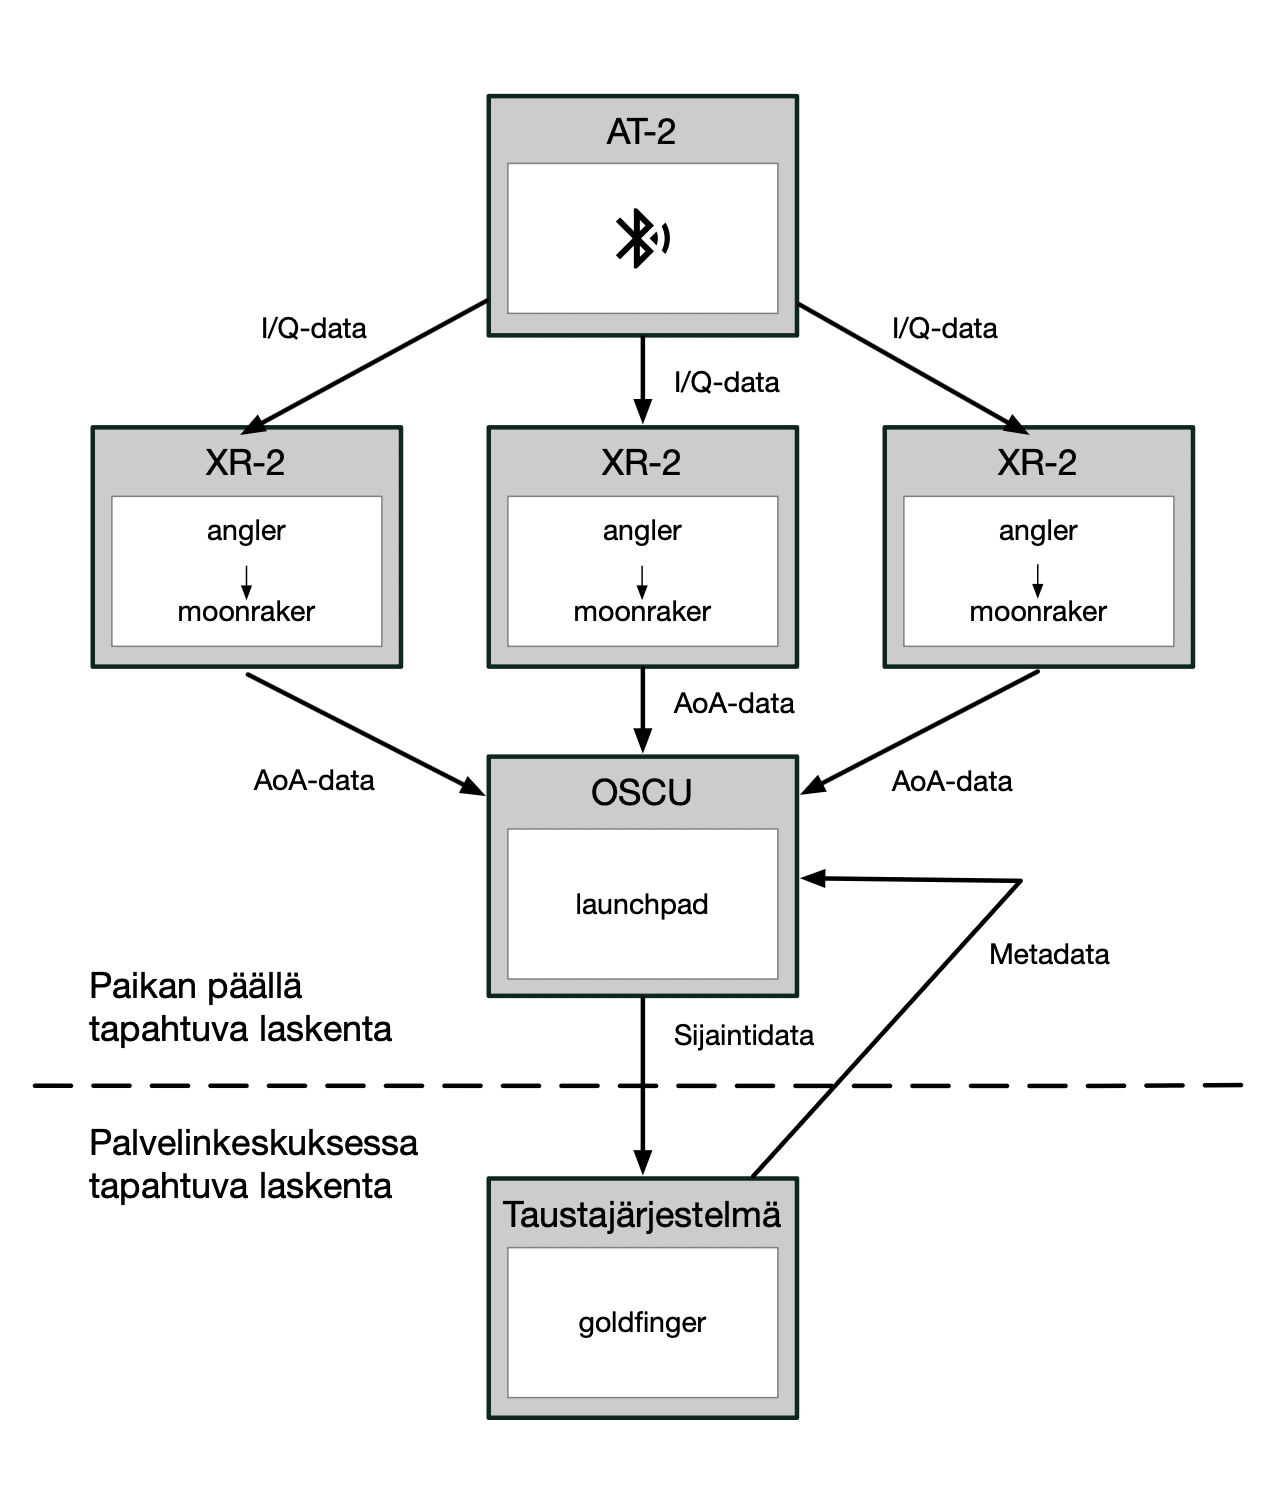
\includegraphics[width=15cm]{jarjestelmaarkkitehtuuri}
\caption{Järjestelmäarkkitehtuuri}
\label{fig:jarjestelmaarkkitehtuuri}
\end{figure}

Tässä luvussa keskitytään \emph{launchpad}-sovelluksen hyödyntämään paikannusalgoritmiin, mutta sitä ennen käsitellään lyhyesti tulokulman laskentamenetelmät sekä \emph{angler}-sovelluksen toiminta. Tekijänoikeussyistä tutkielmassa ei hyödynnetä Go-ohjelmointikielellä toteutettua ohjelmakoodia. Sen sijaan algoritmi on toteutettu R-ohjelmointikielellä.

\subsection{AoA-menetelmistä}

vaihe-eron havaitsemiseen.

\emph{MUSIC-algoritmi} esitys seuraa Monson H. Hayesin kirjaa \emph{Statistical Digital Signal Processing and Modeling} (1996) \citep{Hayes-1996}.

Gunia \citep{Gunia-2023}

Lisäksi \emph{angler}-sovellus hyödyntää niin ikään omaa hiukassuodinalgoritmiaan tulokulmien laskentaan. Tätä hiukassuodinalgoritmia ei käsitellä tämän tutkielman puitteissa.

\subsection{Kalibraatioalgoritmi}

Koska \emph{angler}-sovellus laskee suuntimakulman aina antennielementin määrätystä reunasta nähden, on tärkeää, että laitteen asemointi karttapohjoiseen nähden on tiedossa. Koska laitteen tarkan kulman arvioiminen asennusympäristössä on haastavaa eikä laite sisällä kompassia, on alla esitetty SIR-hiukassuodinta hyödyntävä kalibraatioalgoritmi, joka ottaa huomioon myös laitteen intertiamittausyksiköstä saatavat kallistumis- ja nyökkäämiskulmat. Kalibraatio-ongelma on esitetty kaaviossa TODO.

\begin{algorithm}[H]
\label{kalibraatioalgo}
\DontPrintSemicolon
\SetAlgoShortEnd
\KwResult{Posteriorisiloitinjakauman $p(x_{k}|y_{1:T})$ estimaatti.\;}
\KwData{Suodinjakaumia edustavat hiukkaset ja näihin liittyvät painot ${w_k^i, x_k^i}$, missä $i=1,\ldots,N$ ja $k=1,\ldots,T$\;}
\Begin{
  \Begin{Asetetaan $w_{T|T}^i = w_T^i$, jokaiselle $i=1,\ldots,N$;}
  \For{$k=\{T-1,\ldots,0\}$}{
    \Begin{Lasketaan uudet painot \newline $w^i_{k|T} = \sum_j w_{k+1|T}^j  \frac{w_k^i p(x_{k+1}^j|x_k^i)}{\sum_l w_k^l p(x_{k+1}^j|x_k^l)}$\;}
  }  
}
\caption{Kalibraatioalgoritmi}
\end{algorithm}

,

\section{Datan kuvaus}

Koeasetelmaa varten AT-2-tagi on asetettu lähettämään IQ-dataotoksia 20hz taajuudella. AZIMUTH AND ELEVATION AND THEIR DISTRIBUTIONS. Nämä on kuvattu tarkemmin osiossa TODO. Jokaisen XR-2-laitteen \emph{angler}-sovellus laskee näiden perusteella sekvenssinumeron, jonka perusteella samasta AT-2-tagin lähettämästä IQ-dataoksesta lasketut usean eri vastaanottimen laskemat tulokulmat voidaan yhdistää samaan IQ-dataotokseen. XR-2-laitteen lähettämä tulokulmadata on kuvattu alla.

\def\arraystretch{1.25} 
\begin{table}[H]
\centering
\begin{tabular}{|l|l|l|}
\hline
Muuttuja & Kuvaus & Esimerkkiarvo\\
\hline
id & havainnon yksilöivä tunniste & 317,092 \\
ts & havainnon aikaleima & 2024-04-08 21:38:20.998+00\\
locator\_mac & XR-2-laitteen MAC-osoite & 2c:e3:10:00:07:a6
\\
asset\_tag\_mac & AT-2-tagin MAC-osoite & 2c:e3:10:00:63:89\\
sequence\_nr & \makecell[l]{kulmadatan IQ-dataotokseen yhdistävä \\ juokseva numerointi} & 2,066\\
azimuth\_location & \makecell[l]{atsimuuttikulman $\theta$ \\ jaukauman sijaintiparametri (radiaania)} & 0.39
\\
azimuth\_scale & \makecell[l]{atsimuuttikulman $\theta$ \\ jaukauman skaalaparametri ($\frac{1}{\text{radiaania}^2}$)} & 80.98
\\
elevation\_location & \makecell[l]{korkeuskulman $\gamma$ \\ jaukauman sijaintiparametri (radiaania)} & 0.13
\\
elevation\_scale & \makecell[l]{korkeuskulman $\gamma$ \\ jaukauman skaalaparametri ($\text{radiaania}^2$)} & 0.012
\\
quality\_sndr & signaali-kohinasuhde & 22.0 \\
rssi & signaalin vahvuus (dBm) & -81\\
distance & arvioitu etäisyys lähettimeen (m) & 18.6\\
\hline
\end{tabular}
\caption{Tulokulmamuuttujat}
\label{tab:aoa-muuttujat}
\end{table}

Etäisyys on estimoitu signaalin vahvuudesta käyttäen propagaatiomallia. Etäisyyttä tai signaalin vahvuutta ei käytetä paikantamiseen, joten tämän mallin käsittely jätetään tutkielman ulkopuolelle. Munoz (2009) luku 2 sisältää yleiskatsauksen propagaatiomalleista. \citep{Munoz-2009}

\emph{launchpad}-sovelluksessa tulokulmadataan yhdistetään XR-2-laitteen MAC-osoitteen perusteella lisäksi tarvittavaa, XR-2-laitteita koskevaa metadataa. Näihin kuuluvat laitteen korkeus, laitteen suuntimakulma ja karttakoordinaatit. Metadata on kuvattu taulukossa \ref{tab:metadata}.

\def\arraystretch{1.25} 
\begin{table}[H]
\centering
\begin{tabular}{|l|l|l|}
\hline
Muuttuja & Kuvaus & Esimerkkiarvo\\
\hline
locator\_mac & XR-2-laitteen MAC-osoite & b8:27:eb:66:0d:2a\\
lat & vastaanottimen sijainti (leveyspiiri) & 60.448265\\
lon & vastaanottimen sijainti (pituuspiirit) & 22.294823\\
direction & suuntimakulma $\eta$ (astetta) & 34\\
height & vastaanottimen korkeus (m) & 2.22 \\
\hline
\end{tabular}
\caption{Metadata}
\label{tab:metadata}
\end{table}

Atsimuuttikulma \(\phi\) lasketaan aina vastaanottimen tietyltä sivulta, joten se vastaa napapohjoista ainoastaan siinä tapauksessa, että vastaanottimen kyseinen sivu on asetettu kohtisuoraan napapohjoiseen nähden. Käytännössä vastaanottimien asettaminen tiettyyn kulmaan ei ole aina mahdollista eikä vaihe-erojen mittaamisen kannalta edes suotavaa. Tämän vuoksi jokaiselle vastaanottimelle on tietokantaan tallennettu oma suuntimakulma \(\eta\). Toisin kuin tulokulmadatan kulmat, on tämä tallennettu tietokantaan asteina. Kokeessa käytetään napapohjoisesta laskettuja kulmia \(\Phi\), jotka lasketaan jokaiselle havainnolle havainnon vastaanottimen suuntimakulman avulla

\begin{align}
\Phi=(\theta + \eta \times \frac{\pi}{180^\degree}) \mod 2 \pi.
\end{align}.

Suuntimakulma \(\Phi\) kertoo vastaanottimen ja lähettimen välisen kulman. Lisäksi saatavilla on PostGIS-muotoon tallennettua polygonidataa, joka vastaa koeympäristön pohjapiirrustusta sekä koeympäristössä esiintyviä liikkumisen estäviä kohteita, kuten hyllyjä tai pöytiä. Näitä hyödynnetään sekä sijaintialgoritmin alustuksessa että karttasovitusalgoritmissa (kts. TODO)

Havaintomuuttujien ohella koetilanteesta on tallennettu testipolku, jota pitkin AT-2-tagia liikutetaan koetilanteessa. Testipolkudata pitää sisällään karttaan piirretyn janan pääte- ja sisäpisteet. Tallennettu sijainti perustuu koeympäristön lattiaan pohjapiirrustusten sekä laser-mittausten avulla tehtyihin merkintöihin. Näin saadut testimuuttujat on kuvattu taulukossa (\ref{tab:testimuuttujat}).

\def\arraystretch{1.25} 
\begin{table}[H]
\centering
\begin{tabular}{|l|l|l|}
\hline
Muuttuja & Kuvaus & Esimerkkiarvo\\
\hline
path\_lat & polkupisteen sijainti (leveyspiiri) & 60.44819 \\
path\_lon & polkupisteen sijainti (pituuspiiri) & 22.29493 \\
\hline
\end{tabular}
\caption{Testimuuttujat}
\label{tab:testimuuttujat}
\end{table}

\noindent Testimuuttujia käytetään paikannusalgoritmien paikannusvirheen laskemisessa.

\subsection{Karttaprojektioista}

Kaikki yllä esitetyssä datassa esiintyvät sijaintikoordinaatit on tallennettu tietokantaan WGS 84 -tasokoordinaattijärjestelmässä. Koska hiukassuotimiin perustuvaa paikannusalgoritmia sovellettaessa on monin paikoin tarve syöttää parametereja metrijärjestelmässä. Tästä syystä leveys- ja pituusasteisiin perustuvat koordinaatit muunnetaan laskentaa varten metreiksi ja metreinä esitetyt sijaintitulokset muutetaan tulosten esittämistä varten takaisin WGS 84 -koordinaattijärjestelmään.

Muunnos tapahtuu lineaarisella interpolaatiolla. Määritellään ensin kerrospolygonin rajausalue. Koska kaikki käytetyt koordinaatit ovat tämän rajausalueen sisällä, voidaan tätä rajausaluetta käyttää konversiossa metreiksi. Rajausalue koostuu neljästä kulmapisteestä. Poimitaan näistä pisteistä minimit ja maksimit sekä pituus- että leveyskoordinaateille. Näin saadaan neljä arvoa \(B_{\text{lonlat}}=\{\text{lon}_{\text{min}}, \text{lon}_{\text{max}}, \text{lat}_{\text{min}}, \text{lat}_{\text{max}}\}\). Määritellään rajausalueen sivujen pituus metreinä geodeettisen etäisyyden avulla, jolloin saadaan kaksi metreissä laskettua etäisyyttä \(D_{\text{m}}={d_{\text{lon}}, d_{\text{lat}}}\) . Käytetään näitä kulmapisteitä sekä metreinä laskettuja etäisyyksiä interpoloimaan koordinaatit WGS 84 -koordinaattijärjestelmästä metreissä esitetyille arvoalueille \([0, \text{max}(x_m)]\) ja \([0, \text{max}(y_m)]\) seuraavasti:

\begin{align}\label{wgs84-m}
x_m = f(x_{\text{lon}}; B_{\text{lonlat}}, D_m) = \frac{x_{\text{lon}} -\text{lon}_{\text{min}}}{\text{lon}_{\text{max}}-\text{lon}_{\text{min}}} \times d_{\text{lon}}   \\
y_m = f(y_{\text{lat}}; B_{\text{lonlat}}, D_m) = \frac{y_{\text{lat}} -\text{lat}_{\text{min}}}{\text{lat}_{\text{max}}-\text{lat}_{\text{min}}} \times d_{\text{lat}}
\end{align},

missä \(x_m\) vastaa leveyskoordinaatteja metreissä ja \(y_m\) pituuskoordinaatteja metreissä. Vastaavasti käännös takaisin WGS 84 -koordinaattijärjestelmään tapahtuu vastaavasti:

\begin{align}\label{m-wgs84}
x_{\text{lon}} = f(x_m; B_{\text{lonlat}}, D_m) = \frac{x_{\text{m}}}{d_{\text{lon}}} \times (\text{lon}_{\text{max}}-\text{lon}_{\text{min}}) + \text{lon}_{\text{min}} \\
y_{\text{lat}} = f(y_m; B_{\text{lonlat}}, D_m) = \frac{y_{\text{m}}}{d_{\text{lat}}} \times (\text{lat}_{\text{max}}-\text{lat}_{\text{min}}) + \text{lat}_{\text{min}}
\end{align}.

\subsection{Muunnettu data}

Kun yllä esitetyt konversiot on. Käytetään datassa seuraavia. TÄHÄN NOTAATIOT.

\section{Sisätilapaikannusalgoritmi}

\subsection{Ongelman kuvaus}

Tarkoituksena on estimoida liikkuvan AT-2-tagin sijaintia. Merkitään tätä estimoitavaa tilasarjaa \(x_{1:k}=\{x_1,\ldots,x_k\}\). Lisäksi merkitään \(x_0\) testilaitteen lähtösijaintia. Jokainen tilasarjan havainto koostuu suuntimakulmasta sekä pituus- että leveyskoordinaateista \((x_k^x, x_k^y)\). Määritellään tilalle liikkuvan AT-2-tagin kulkua kuvaava vektorisuunnistukseen (dead reckoning) perustuva malli (\ref{tilamalli-liikkuva})

\begin{align}\label{tilamalli-liikkuva}
x_{k+1}=f(x_k, \nu_k)=x_k+D_k \begin{bmatrix} \cos\psi_k \\ \sin\psi_k \end{bmatrix}+\nu_k,
\end{align}

\noindent missä \(D_k\) on AT-2-tagin ajanhetkenä \(k\) kulkema matka ja \(\psi_k\) AT-2-tagin suuntimakulma kyseisenä ajanhetkenä. \(\nu_k\) on kohinaa, joka syntyy mittausvirheestä ja jolle voidaan olettaa \(\sim \mathcal{N}(\mu_x,\,\sigma_x^{2})\). Jos laite on paikallaan, yksinkertaistuu malli muotoon \(x_{k+1}=f(x_k)=\text{id}(x_k)=x_k\), missä \(\text{id}(\cdot)\) on identiteettifunktio.

Vastaavasti \(y_{1:k}=\{y_1,\ldots,y_k\}\) kuvaa AT-2-tagin ja XR-2-laitteiden välillä laskettuja kulmahavaintoja. Näin ollen jokainen havainto koostuu (maksimissaan) paikantimien määrää vastaavasta määrästä kulmia. Havainnot lasketaan sekunnin tarkkuudella, mutta todellinen havaintotarkkuus on tiheämpi.

\noindent Lisäksi tunnetaan sensoreihin \(\{s^1,\ldots,s^4\}\) liittyvät pituus- ja leveyskoordinaatit \((\lambda, \phi)\), jotka on muutettu TODO mukaan metreiksi.

\begin{align}
u=\begin{bmatrix} \lambda^1 & \phi^1 \\   \vdots & \vdots \\ \lambda^4 & \phi^4 \end{bmatrix}.
\end{align}

Määritellään havainnoille malli

\begin{align}\label{havaintomalli}
y_k=h(x_k, u)+e_k=\text{atan2}(\begin{bmatrix}\phi^1-x_k^y\\ \vdots \\ \phi^4-x_k^y\end{bmatrix}, \begin{bmatrix}\lambda^1-x_k^x\\ \vdots \\ \lambda^4-x_k^x\end{bmatrix})+e_k,
\end{align}

\noindent missä

\begin{align}\label{atan2}
\displaystyle \operatorname{atan2}(y,x)={\begin{cases}\arctan({\frac {y}{x}})&{\text{jos }}>0,\\\arctan({\frac {y}{x}})+\pi &{\text{jos }}<0{\text{ ja }}y\geq 0,\\\arctan({\frac {y}{x}})-\pi & {\text{jos }}>0{\text{ ja }}<0,\\+{\frac {\pi }{2}}&{\text{jos }}x=0{\text{ ja }}>0,\\-{\frac {\pi }{2}}&{\text{jos }}x=0{\text{ ja }}<0,\\{\text{ei määritelty}}&{\text{jos }}x=0{\text{ ja }}y=0\end{cases}}
\end{align}

\noindent ja kohina noudattaa moniulotteista normaalijakaumaa \(e_k\sim\mathcal{N}(0,{\Sigma})\).

Kovarianssimatriisin estimaattina käytetään kunakin ajanhetkenä \(k\) antennikohtaisista havainnoista estimoituja otosvariansseja \(\text{diag}(\hat{\sigma}^1_k,\ldots,\hat{\sigma}^4_k)^2=\text{diag}(\frac{1}{n-1}\sum_{i=1}^n(s_i^1-\bar{s})^2,\ldots,\sum_{i=1}^n(s_i^4-\bar{s})^2)\). Määrittelemätön \(\text{atan2}\)-tapaus, jossa \(x=0\) ja \(y=0\) on käytetyllä mittaustarkkuudella käytännössä mahdoton. Jos tapaus halutaan välttää, voidaan nolla-arvot tarpeen vaatiessa korvata joillakin hyvin lähellä nollaa olevalla arvolla. Saadaan uskottavuusfunktioksi

\begin{align}
p(y_k|x_k)\propto\prod_{j=1}^4\exp\left\{-\frac{\norm{h(x^j_k,u)-y^j_k}^2}{2(\hat{\sigma}_i^j)^2}\right\},
\end{align}

\noindent missä \(j=\{1,l\dots,n\}\) vastaa nyt kutakin XR-2-laitetta. Kumpikaan funktiosta \(h(\cdot)\) ja \(f(\cdot)\) ei ole lineaarinen, joten SIR-algoritmi on sopiva valinta ongelman ratkaisemiseksi. Koetuloksia arvioidaan ensisijaisesti paikannusvirheen avulla. Paikannusvirhe \(e_k\) lasketaan jokaisen ajanhetken \(k\) posteriorijakaumaestimaatista \(\hat{p}_k\) painotettuna keskiarvona

\begin{align}
\epsilon_k = \sum_{i=1}^Nw^k_i d(x^i_k, y_k),
\end{align}.

\noindent missä \(w_i^k\) on ajanketken \(k\) partikkelien normalisoitu paino ja \(d(x^i_k,y_k)\) partikkelien ja testilaitteen todellisen sijainnin välisen etäisyyden laskeva funktio.

\hypertarget{uskottavuusmallit}{%
\subsection{Uskottavuusmallit}\label{uskottavuusmallit}}

Jokainen yhtä tulokulmaa vastaava \emph{angler}-sovelluksen tuottama havaintodatarivi pitää sisällään neljä parametrimuuttujaa, \texttt{azimuth\_location}, \texttt{azimuth\_scale}, \texttt{elevation\_location} ja \texttt{elevation\_scale}. Koska \emph{angler}-sovellus on kirjoitettu varta vasten tuottamaan dataa hiukassuodinpaikannusalgoritmia varten, ovat nämä suoraan hiukassuotimen uskottavuusmallin parametreja.

\emph{Angler}-sovelluksessa XR-2-laitteen ja AT-2-tagin välinen atsimuuttikulma simuloidaan von Mises -jakaumasta, jolloin muuttujat \texttt{azimuth\_location} ja \texttt{azimuth\_scale} vastaavat tämän jakauman sijainti- ja skaalaparametreja \(\mu\) ja \(\kappa\) ja näistä edellistä voidaan pitää itse atsimuuttikulman estimaattina. Määritellään siis jokaiselle hiukkassuotimen aikahetkelle \(k\) sekä XR-2-laitteelle \(l\) seuraava atsimuuttikulman uskottavuusmalli:

\begin{align}\label{atsimuutti-uskottavuusmalli}
L_{\theta_{k,l}}(y_{k,l}|x_{k,l}; \mu_{k,l}, \kappa_{k,l})=\frac{e^{\kappa_{k,l} \text{cos}(x_{k,l}-\mu_{k,l})}}{2 \pi I_0(\kappa_{k,l})}
\end{align},

missä \(I_0\) on 0:s ensimmäisen lajin Bessel-funktio ja \(x_{k,l}\) on jokaisen hiukkasen \(n=1,\ldots,N\) sekä XR-2-laitteen \(l\) välinen suuntimakulma.

Vastaavasti \emph{angler}-sovelluksessa XR-2-laitteen ja AT-2-tagin välinen korkeuskulma simuloidaan katkaistusta normaalijakaumasta, jolle \(a=0\) ja \(b=2 \pi\). Nyt muuttujat \texttt{elevation\_location} ja \texttt{elevation\_scale} vastaavat tämän jakauman sijainti- ja skaalaparametreja \(\mu\) ja \(\sigma^2\) ja näistä edellistä voidaan pitää itse korkeuskulman estimaattina. Määritellään jokaiselle hiukkassuotimen aikahetkelle \(k\) sekä XR-2-laitteelle \(l\) seuraava korkeuskulman uskottavuusmalli:

\begin{align}\label{korkeus-uskottavuusmalli}
L_{\gamma_{k,l}}(y_{k,l}|x_{k,l}; \mu_{k,l}, \sigma^2_{k,l}, a=0, b=2 \pi)=\frac{1}{\sqrt{2 \pi}} \text{exp}(-\frac{(x_{k, l}-\mu_{k, l})}{2 \sigma^2}) / \sqrt{\sigma^2}Z_{k,l}
\end{align},

missä \(Z_{k,l}=\frac{1}{2}(1+\text{erf}(\frac{b-\mu_{k,l}}{\sqrt{\sigma^2}}))-\frac{1}{2}(1+\text{erf}(\frac{a-\mu_{k,l}}{\sqrt{\sigma^2}}))\) ja \(x_{k,l}\) on jokaisen hiukkasen \(n=1,\ldots,N\) sekä XR-2-laitteen \(l\) välinen korkeuskulma.

Uskottavuusmallit \ref{atsimuutti-uskottavuusmalli} ja \ref{korkeus-uskottavuusmalli} kertomalla saadaan yhdistetty uskottavuusmalli hiukkassuotimen aikahetkelle \(k\) sekä XR-2-laitteelle \(l\)

\begin{align}\label{yhdistetty-uskottavuusmalli}
L_{k,l}=L_{\theta_{k,l}} \times L_{\gamma_{k,l}}
\end{align},

josta voidaan edelleen laskea jokaisen hiukkasen uskottavuus ajanhetkenä \(k\)

\begin{align}\label{lopullinen-uskottavuusmalli}
L_{k}=\prod_i^L L_{{k,i}}
\end{align}.

Koska yllä esitettyjen mallien uskottavuudet ovat käytännössä erittäin pieniä, käytetään numeerisista syistä itse algoritmissa logaritmoituja uskottavuusmalleja, jolloin \(l_{k,l} = \text{log}(L_{\theta_{k_l}}) + \text{log}(L_{\gamma_{k_l}})\) ja \(l_k = \sum_i^L l_{k,i}\).

\hypertarget{datan-valinta}{%
\subsection{Datan valinta}\label{datan-valinta}}

In the positioning particle filter, convex hull method is used in angle selection. The basic premise of this method is simple. Before evaluating particle likelihoods an angle/locator selection is performed. As one step of this process, a convex hull is drawn around the particle cloud and only angles that intersect this polygon get included in the likelihood evaluation. The following illustration explains the method.

Here the angles from the locators \#2 and \#1 get included in the likelihood evaluation as they intersect the convex hull of the particle cloud whereas the angle from locator \#3 is discarded.
As the basic interpretation of the particle cloud is that the probability of the tag being within it is one, we can safely assume that the correct position of the tag is also within the convex hull enclosing the particle cloud. Thus this method works well for getting rid of poor angles and reflections.

The Problem
However, the above method also leads to a problem: the smaller the particle cloud gets, the more precise the angles need to be to get included in the likelihood evaluation. When running the positioning particle filter at the frequency of one this is rarely a problem, as this frequency necessitates a noise q value of 1.5m thus leading to particle clouds averaging at least 3m in width. However if we want to move to a higher frequency to be able to reduce the noise value into centimeter range, this will become a problem.

The Solution
The simplest solution to the above problem is to add padding to the convex hull. An example of this is pictured below.

In the R positioning particle filter this padding is achieved by introducing a new design parameter called ch\_q\_adjustment. Before the application of the movement model this value is added to the q noise value and the particles are moved using this adjusted q\_new = q + ch\_q\_adjustment value. The resulting moved particle cloud is then used to create the adjusted convex hull after which these particles are discarded and the original particles are moved again using the plain q value.
This method of achieving the convex hull padding is a bit involved and probably computationally more costly than just applying the movement model once and adjusting the size of the resulting convex hull using some other transformation. However this approach has the upside of retaining the original logic of convex hull creation and allowing to ``decompose'' the used noise. I.e. using a q value of 0.9 and ch\_q\_adjustment value of 0.52 leads to a similar sized convex hull as using the q value of 1.42.

\hypertarget{dynaaminen-malli}{%
\subsection{Dynaaminen malli}\label{dynaaminen-malli}}

Dynaamisen mallin tehtävänä on liikuttaa hiukkasia ajanhetkien \(k\) ja \(k+1\) välillä. Dynaaminen malli perustuu vektorisuunnistusmalliin \ref{tilamalli-liikkuva}. Koska AT-2-tagi ei sisällä luotettavaa IMU-yksikköä, ei tagi tuota nopeus- tai suuntadataa. Tästä syystä vektorisuunnistusmallin nopeutta ilmaiseva skalaarimuuttuja \(D_k=0\), jolloin malli yksinkertaistuu satunnaiskävelymalliksi

\begin{align}\label{dynaaminen-malli-empiirinen}
x_{k+1}=x_k + v_k
\end{align},

missä \(v_k\) on kohinaa. Kohina luodaan jokaiselle ajanhetkelle seuraavasti. Ensin luodaan etäisyysvektori \(d_k\) katkaistusta normaalijakaumasta, jonka sijaintiparametri on 0 ja missä keskihajonta \(q\) ja katkaisukohdat \(q_min\) sekä \(q_max\) ovat paikannusalgoritmin suunnitteluparametreja:

\begin{align}
&d_k \sim \mathcal{N_{\text{katkaistu}}}(\mu=0, \sigma=q, a=q_{\text{min}}, b=q_{\text{max}}),
\end{align}.

Tämän jälkeen luodaan suuntavektori \(p\) tasajakaumasta

\begin{align}
&p_k\sim\mathcal{U}(0, 2 \pi)
\end{align},

ja lopulta kohinavektori

\begin{align}
&v_k = (\text{cos}(p_k) \times d_k, \text{sin}(p_k) \times d_k)
\end{align},

missä vektorin ensimmäinen elementti vastaa sijaintien leveysasteiden kohinaa ja toinen elementti pituusasteiden kohinaa.

\hypertarget{paikallaanolon-havaitseminen}{%
\subsubsection{Paikallaanolon havaitseminen}\label{paikallaanolon-havaitseminen}}

Paristonsäästyösyistä AT-2-tagi lähettää dataa ainoastaan liikkuessaan. Jos laite ei ole 10 sekunnin aikana havainnut IMU-yksikön perusteella kiihtyvyyttä, lopettaa laite datan lähettämisen. Laite on tällöin valmiusmoodissa. Tätä tietoa voidaan hyödyntää poistamalla dynaamisesta mallista kohina, kun laitteen tiedetään olevan paikallaan. Koska hiukkassilottimen (kts. kohta TODO) vuoksi tarvitsemme paikannusalgoritmiin viipeen, voimme hyödyntää tätä viivettä myös paikallaolon tehokkaampaan havaitsemiseen.

Jos yksikään XR-2-laite ei ole havainnut tagia yhdenkään sekuntiin kuuluvan 20 aika-askeleen aikana, voimme olettaa laitteen olevan valmiusmoodissa ja siten myös paikoillaan. Huomattavaa on kuitenkin, että päinvastainen ei päde. Paikoillaan oleva laite ei välttämättä ole valmisumoodissa, sillä valmiusmoodiin siirtyminen kestää 10 sekuntia. Tähän oletukseen perustuen voidaan havaita paikallaolon ja vaimentaa dynaamista mallia algoritmin \ref{paikallaanoloalgo} avulla. Algoritmi ajetaan jokaisella aika-askeleella \(k\) ennen hiukkasten siirtoa dynaamisen mallin avulla.

\begin{algorithm}[H]
\label{paikallaanoloalgo}
\DontPrintSemicolon
\SetAlgoShortEnd
\KwResult{Positiivinen kokonaislukumuuttuja $m$, joka osoittaa kuinka moneksi aikahetkeksi dynaamista mallia tulee vaimentaa. Jos $m=0$ mallia ei vaimenneta.;}
\KwData{Tagin tulokulmadata $n+1$ aika-askeleelle (nykyinen aika-askel + $n$ aika-askelta tulevaisuuteen). $n$ tulee asettaa niin, että paikallaan oleva tagi ehtii valmiustilaan. Koska tämä tapahtuu 10 sekunnin kohdalla, valitaan $n=200$. Jos saatavilla, edellinen muuttujan $m$ arvo. Algoritmin ensimmäisellä ajokerralla asetetaan $m=0$;}
\Begin{
  \Begin{Jos $m>0$, asetetaan $m=f(m)=m-1$ ja pysäytetään algoritmi. Jos $m=0$ jatketaan algoritmin suorittamista.;}
  \For{$k=\{T-1,\ldots,0\}$}{
    \Begin{Lasketaan uudet painot \newline $w^i_{k|T} = \sum_j w_{k+1|T}^j  \frac{w_k^i p(x_{k+1}^j|x_k^i)}{\sum_l w_k^l p(x_{k+1}^j|x_k^l)}$\;}
  }  
}
\caption{Paikallaanolon havaitsemisalgoritmi}
\end{algorithm}

,

What this does is it finds the first missing data time step and sets the m value correspondingly. If there are consecutive missing data time steps this sets m to correspond to the last of these time steps.

Steps: If m==0 apply step 2, otherwise decrement m by 1.
t is the current time step. For each time step l = t+1 \ldots{} t+n do the following:
Check if there is data available for that time step. If not
and m==0 set m=l-t. If m\textgreater0 and m+1==l-t set m=l-t if.
If m!=0 for each application of the movement model for this iteration of the positioning particle filter, adjust the noise q value as follows: q = q/10 (can be adjusted, but we still want to allow for some movement to let the positioning system converge to the right stationary position).

\hypertarget{karttasovitusalgoritmi}{%
\subsubsection{Karttasovitusalgoritmi}\label{karttasovitusalgoritmi}}

Dynaamista mallia sovellettaessa, voimme myös höydyntää saatavilla olevaa sisätilan karttadataa. Hyödynnetään polygoneja ja raycastingia. Asetetaan esimerkiksi rangaistus 1/1000. Jolloin uskottavuusfunktiot muuttuvat muotoon. Toteutus seuraa paperia XYZ (2019 tjsp).

\hypertarget{reitinhakualgoritmi}{%
\subsubsection{Reitinhakualgoritmi}\label{reitinhakualgoritmi}}

\begin{itemize}
\tightlist
\item
  Create separate grids for raw positions and Kalman filtered positions with separate and adjustable grid cell widths.
\item
  After positioning estimates and their Kalman filtered counterparts are created, snap these to the grid. Note! By default particles are not snapped to the grid, only the position estimates.
\item
  See if the previous position is within speed limit / Kalman filter speed limit (these are separate arguments) distance. These are set to 3m/s by default.
\item
  If the speed limit is not exceeded, create a new grid-snapped position. Also create a position to all the grid cells between the newly created position and the previous position. This path is found using A* algorithm.
\item
  If the speed limit is exceeded, wait for new raw / Kalman filtered positions to come in until the speed limit is no longer exceeded, in which case proceed as in the previous step.
\item
  Note! Pathfinding positions are not used anywhere else in the R positioning algorithm. Thus both the pathfinding positions and their Kalman filtered counterpresents create an entirely independent layer of positions on top of raw / Kalman filtered positions.
\item
  Note\^{}2! When doing the A* pathfinding the time between positions is split equally so that the interpolated positions get a fractional time step between the start and stop positions of the pathfinding. Thus the positioning frequency of 1 is not respected.
\end{itemize}

\hypertarget{siloittelualgoritmit}{%
\subsection{Siloittelualgoritmit}\label{siloittelualgoritmit}}

Hyödynnetään alaluvussa TODO esitetty prediktiivistä siloitinta. Satunnaiskulkumalli ei ole optimaalinen, mutta \ldots{}

\subsection{WB-sisätilapaikannusalgoritmi}

Alla esitetään

\begin{algorithm}[H]
\label{wb-positioning}
\DontPrintSemicolon
\SetAlgoShortEnd
\KwResult{Posteriorisiloitinjakauman $p(x_{k}|y_{1:T})$ estimaatti.\;}
\KwData{Suodinjakaumia edustavat hiukkaset ja näihin liittyvät painot ${w_k^i, x_k^i}$, missä $i=1,\ldots,N$ ja $k=1,\ldots,T$\;}
\Begin{
  \Begin{Asetetaan $w_{T|T}^i = w_T^i$, jokaiselle $i=1,\ldots,N$;}
  \For{$k=\{T-1,\ldots,0\}$}{
    \Begin{Lasketaan uudet painot \newline $w^i_{k|T} = \sum_j w_{k+1|T}^j  \frac{w_k^i p(x_{k+1}^j|x_k^i)}{\sum_l w_k^l p(x_{k+1}^j|x_k^l)}$\;}
  }  
}
\caption{Uudelleenpainottava hiukassiloitin}
\end{algorithm}

,

algoritmin ominaisuuksista.

Koeasetelmassa käytetty SMC-algoritmi on toteuttu R-kielellä. Algoritmin toteutus on pääosin vektorisoitu ja tehokas. For-silmukkaa on käytetty ainoastaan ajanhetkien läpikäyntiin. Koska tämän silmukan muuntaminen vektorisoituun muotoon ei ole mahdollista, voidaan toteutusta pitää näiltä osin hyvin optimoituna. Algoritmin datan käsittely on toteutettu täysin suorituskyvyltään erinomaisella \texttt{data.table}-kirjastolla. Koodin profilointi XXX.

Koska algoritmin uskottavuudet sekä painot ovat hyvin pieniä, on laskentatarkkuusongelmien välttämiseksi toteutuksessa käytetty logaritmoituja painoja ja uskottavuusfunktiota. Tämä ei vaikuta lainkaan itse algoritmin toimintaan, mutta estää numeeristen ongelmien syntymisen. Tilanteessa, jossa tietyn paikantimen ja kaikkien partikkelien välinen uskottavuus on nolla, päätyvät kaikki painot nolliksi eikä algoritmi enää toimi. Tällaisessa tilanteessa uskottavuusfunktion R-toteutus kutsuu itseään rekursiivisesti uudelleen niin, että kyseinen paikannin on tiputettu havainnoista.

Paikannusvirheen laskemisessa on etäisyysfunktiona \(d(\cdot)\) käytetty \texttt{raster}-kirjaston \texttt{pointDistance()}-funktiota. Koodissa on korostettu tiiviyden sijaan luettavuutta ja koodi on kommentoitu kattavasti. SMC-algoritmifunktion sekä uskottavuusfunktion R-koodit löytyvät osoitteesta \url{https://github.com/rintakumpu/luk}, mistä löytyy myös asetelmassa käytetty data csv-muodossa sekä kokeen muun koodin sisältävä R Markdown -notebook.

\section{Empiirinen esimerkki}

\subsection{Koeasetelma}

Koetta varten käytettiin yhden minuutin aikana kertyneitä havaintoja. Havaintoja on datassa yhteensä \(N_{obs}=15018\) kappaletta. Havaintojen aikaleimat on tallennettu sekunnin tuhannesosan tarkkuudella.

Esimerkissä käyteteään SMC-algoritmia Bluetooth-paikannussovelluksessa lähettimen sijainnin laskemiseen. Paikannukseen käytettävä data kerättiin toimistoympäristössä Bluetooth Low Energy (BLE) -lähettimen sekä kattoon sijoitettujen vastaanottimien avulla. Havainnot koostuvat vastaanottimien lähettimien signaalien perusteella laskemista, BLE5.1-standardin mukaisista signaalin tulokulmista eli AoA-havainnoista (angle of arrival). Lopuksi esimerkissä analysoidaan ja vertaillaan algoritmin eri versioiden suorituskykyä sekä suorituskyvyn että paikannustarkkuuden näkökulmasta. Vertailuarvona käytetään perinteistä triangulaatio-algoritmia.

Paikaunnusesimerkissä lähettimenä toimi 25 Bluetooth-paikannustagista koostuva Walkbase Foculator -testilaite (kuva \ref{fig:foculator}), vastaanottimena toimistoympäristöön asennetut neljä Walkbase XR-2 -vastaanotinta (kuva \ref{fig:xr2}). Jokainen vastaanotin sisältää kuusitoista antennia, joiden vastaanottamien lähetinsignaalien perusteella vastaanottimet laskevat signaalin tulokulman suhteessa vastaanottimeen. Tarkka tulokulmien laskemiseen käytetty algoritmi on paikantimen antennit toimittaneen Silicon Laboratories, Inc.~-yrityksen liikesalaisuus, mutta perusperiaate on arvioida tulokulma mittaamalla eri antenneiden välistä vaihe-eroa ns. IQ-signaalin avulla.

Esteettömässä ympäristössä koeasetelmassa käytetyn järjestelmän kulmavirhe on hyvin pieni ja paikannusongelma voidaan ratkaista riittävällä tarkkuudella suoraan triangulaatio-algoritmilla. Tässäkin tilanteessa voi paikannusta parantaa suodattimen käytöllä, mutta jo triangulaatio-algoritmin perusversio tuottaa halutun tarkkuuden. Toimistoympäristö on kuitenkin haastava, sillä erityisesti näyttöruudut sekä heijastavat että estävät radiosignaaleja. Silicon Labs lupaa omalle AoA-järjestelmälleen vastaavassa toimisympäristössä (seitsemällä paikantimella) kulmavirheen välillä \(3.7^\degree-5.7^\degree\). Tämä ei kuitenkaan riitä johdonmukaisesti haluttuun alle metrin paikannustarkkuuteen, joten AoA-paikannus toimistoympäristössä tarjoaa hyvän motivaation SMC-menetelmien käytölle.

\begin{multicols}{2}
\begin{figure}[H]
\centering
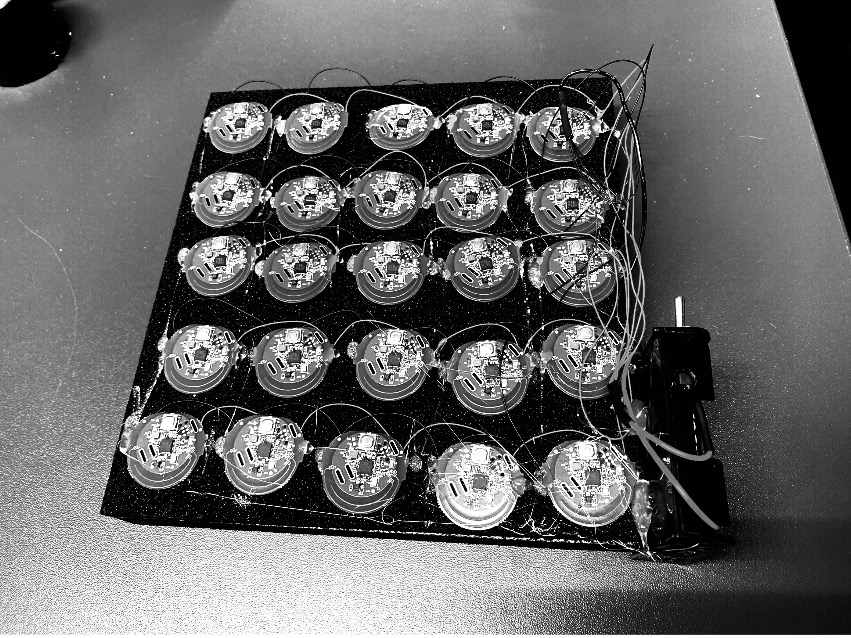
\includegraphics[width=7cm]{foculator}
\caption{Walkbase Foculator}
\label{fig:foculator}
\end{figure}

\begin{figure}[H]
\centering
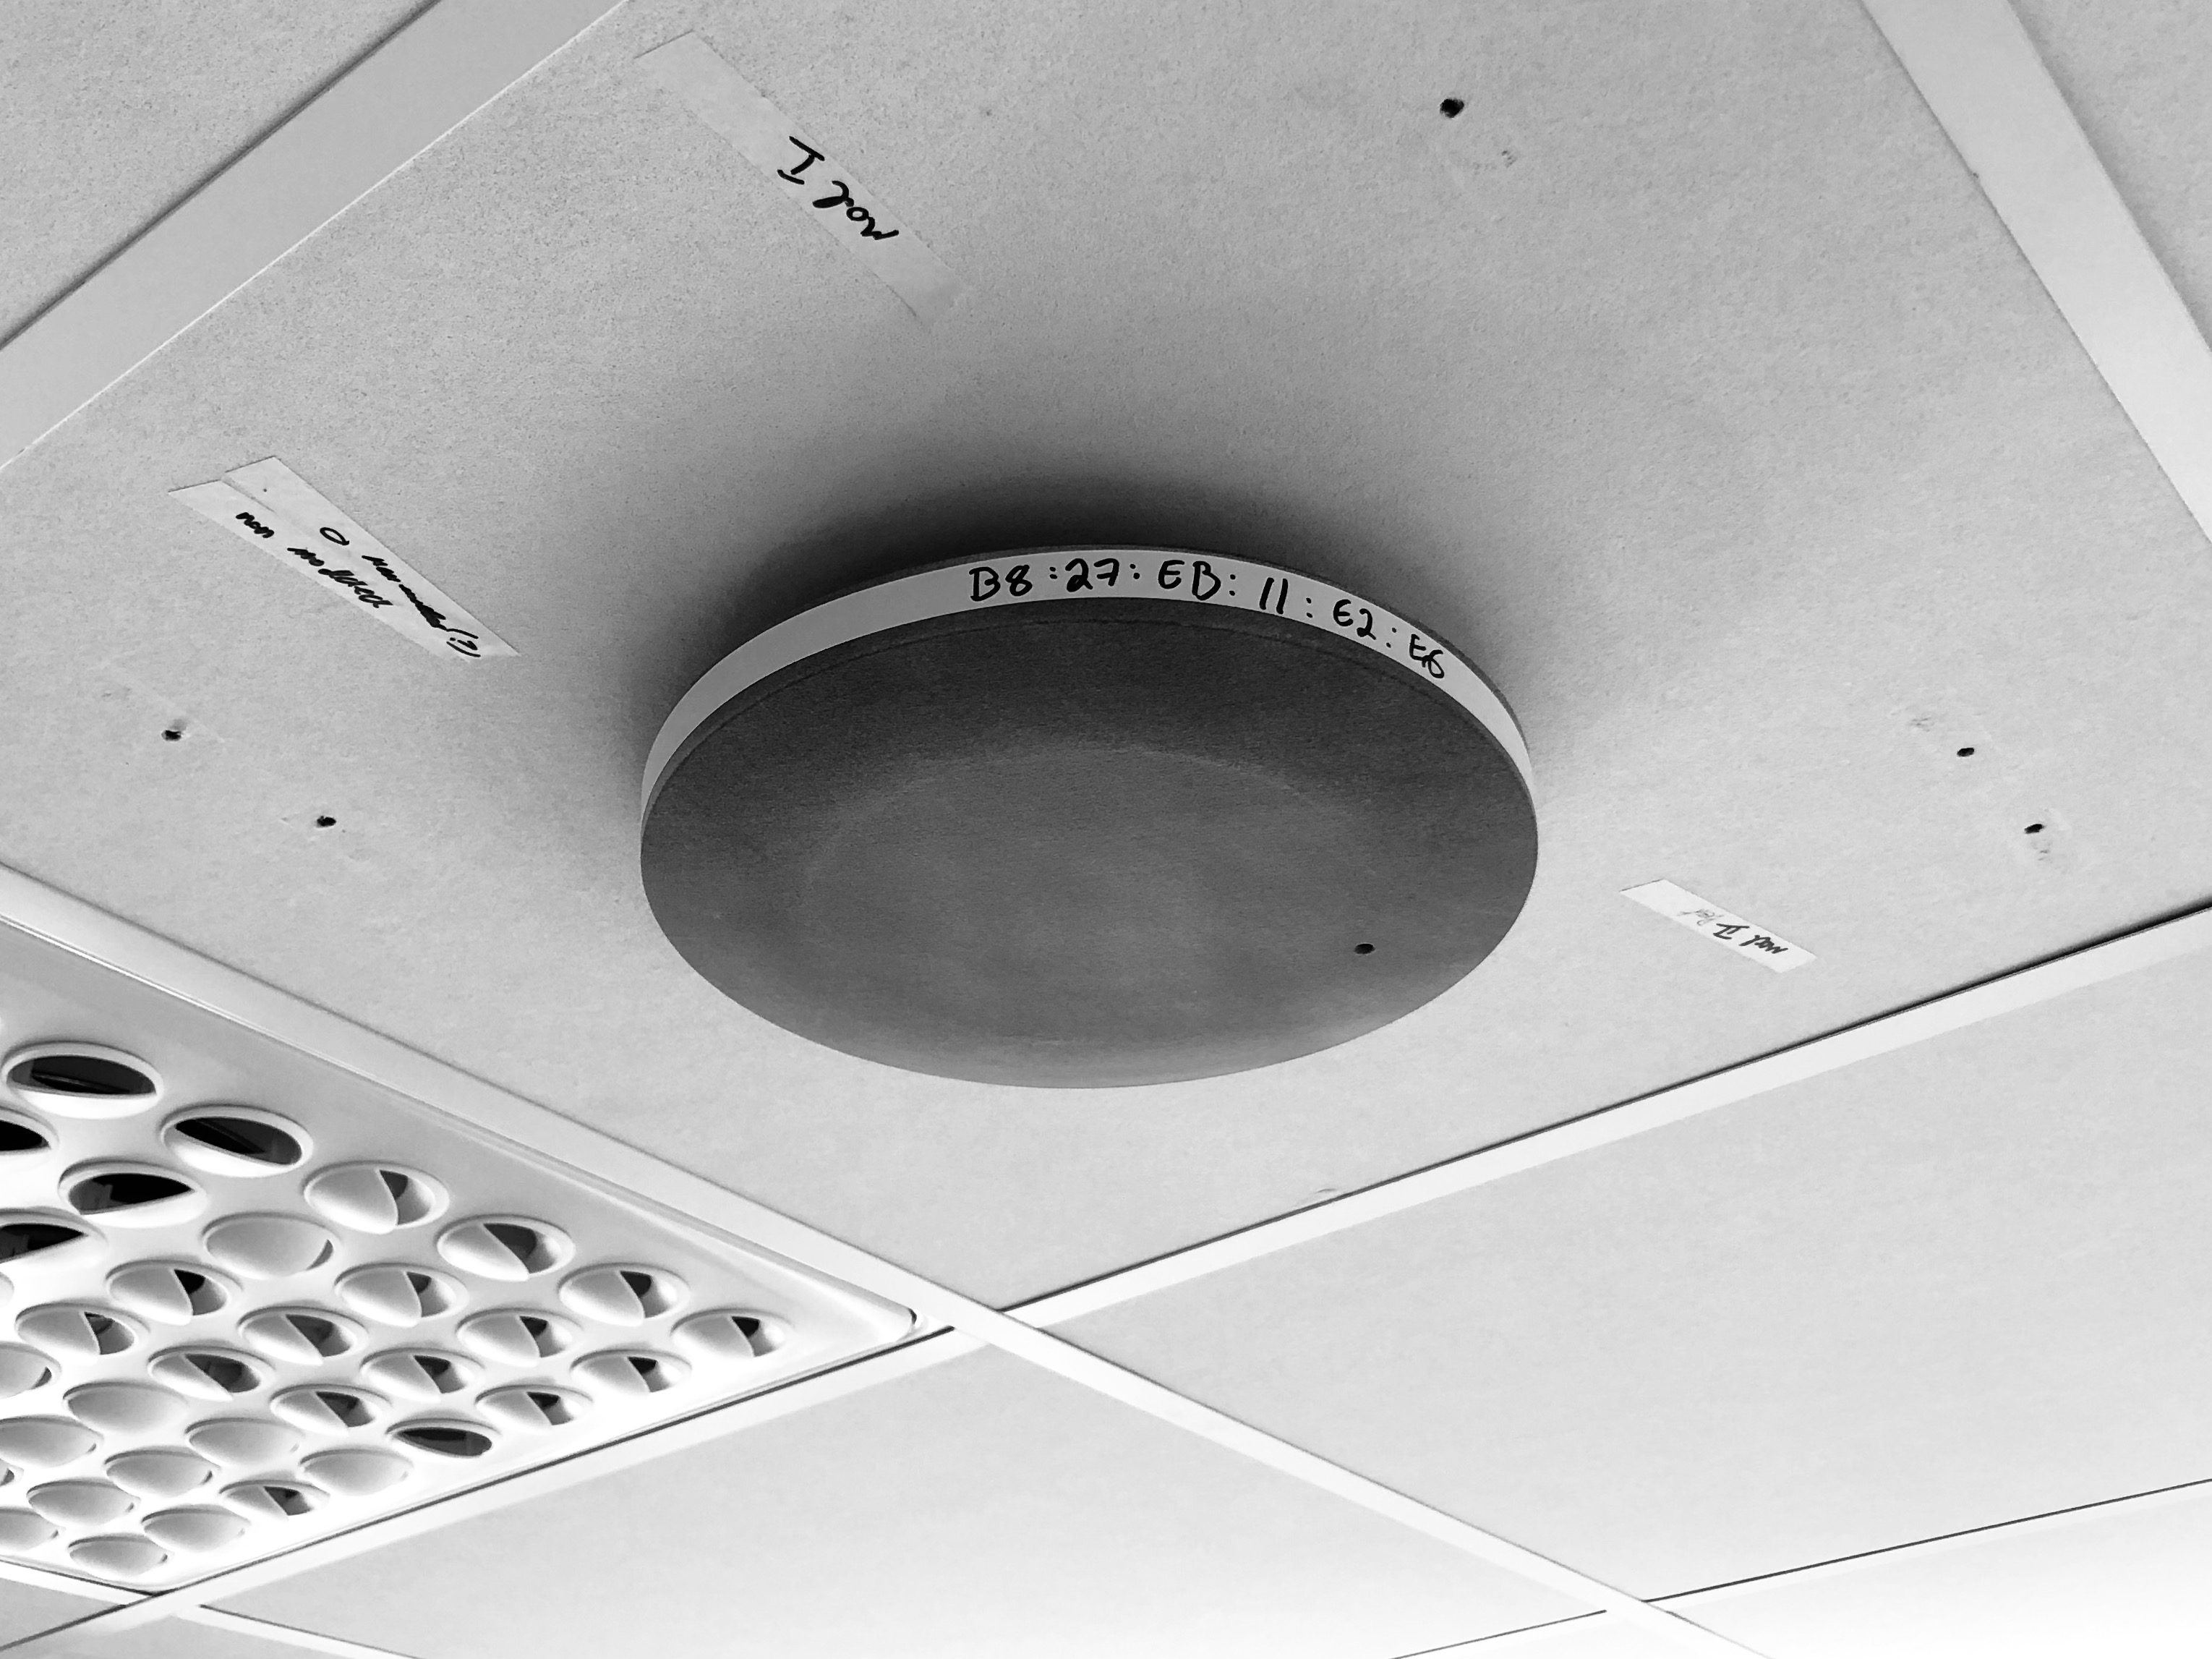
\includegraphics[width=7cm]{xr_2}
\caption{Walkbase XR-2}
\label{fig:xr2}
\end{figure}
\end{multicols}

Data on kuvattu tarkemmin alaluvussa 5.2. Koeympäristön pohjapiirustus on esitetty kuvassa \ref{fig:pohjapiirustus}. Piirustuksessa XR-2-paikantimet on kuvattu punaisilla numeroiduilla ympyröillä. Foculator-testilaitteen sijainti on kuvattu sinisellä ympyrällä. Toimistoympäristön pohjapiirustus on kuvattu harmaalla niin, että piirustuksesta erottuvat toimiston väliseinät.

\begin{figure}[H]
\centering
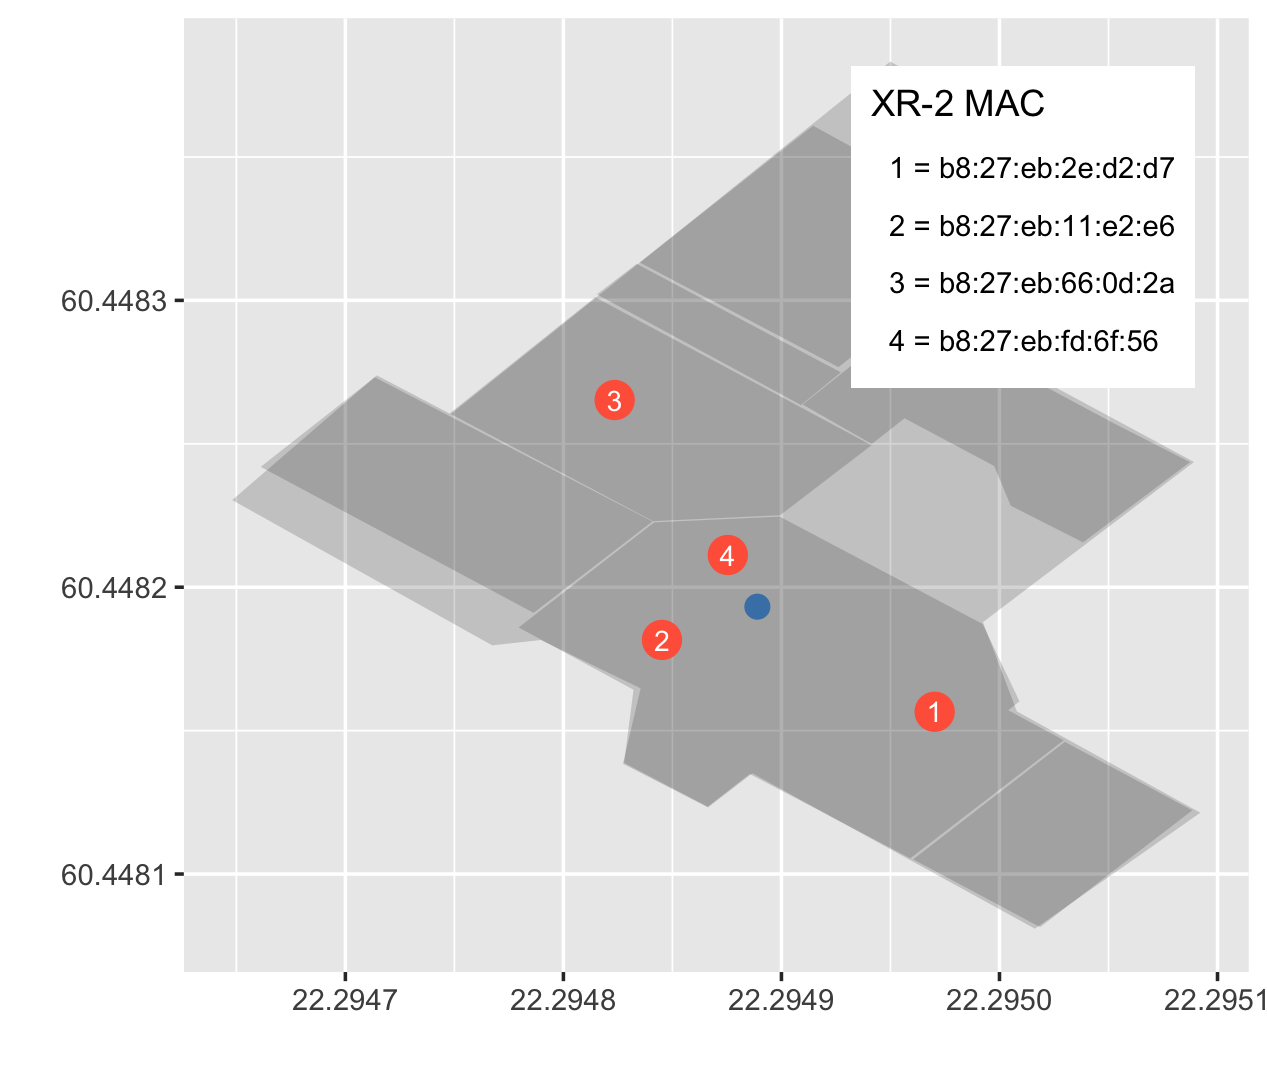
\includegraphics[width=12cm]{office_map}
\caption{Koeasetelman pohjapiirustus}
\label{fig:pohjapiirustus}
\end{figure}

\noindent Toimisto valittiin testiympäristöksi, koska siellä testaaminen on helpompaa ja halvempaa kuin aidossa kauppaympäristössä. Lisäksi toimistossa hyvin toimiva järjestelmä todennäköisesti toimii sellaisenaan vähemmän esteisessä kauppaympäristössä.

Dataa kerättiin sekä liikkuvalla että paikallaan olevalla testilaitteella. Paikallaan oleva testilaite asetettiin pöydälle 1.5 metrin korkeudelle. Liikkuvassa tapauksessa testilaite kiinnitettiin robottiin, joka oli ohjelmoitu seuraamaan haluttua liikerataa vastaavia lattiamerkintöjä ennalta määrätyllä vakionopeudella. Yksinkertaisuuden vuoksi tässä tutkielmassa tarkastellaan ainoastaan ongelmaa, jossa testilaite on paikoillaan. Esitetyt mallit soveltuvat kuitenkin myös liikkuvalle laitteelle. Data kerättiin yöaikaan, jolloin toimiston käyttöaste oli alhainen. Tällä minimoitiin radiosignaalien tielle osuvien ihmisten vaikutus signaaleihin. Maan pinnan kaarevuus on otettu huomioon koeasetelmassa pisteiden välisiä etäisyyksiä laskettaessa.

\subsection{Parametrien valinta}

Priorijakaumana \(p_{x_0}\) käytettiin kahta toisistaan riippumatonta otosta tasajakaumista, joista toinen vastasi leveys- ja toinen pituusasteita. Jakaumien alkupisteet valittiin niin, että ne vastasivat pienimpiä paikantimien leveys- ja pituusasteista. Vastaavasti päätepisteet valittiin niin, että ne vastasivat suurimpia paikantimien leveys- ja pituusasteita.

\begin{align}
&p_{x_{0_{\text{lon}}}}\sim\mathcal{U}(\min{\lambda},\max{\lambda}),\\
&p_{x_{0_{\text{lat}}}}\sim\mathcal{U}(\min{\phi},\max{\phi}).
\end{align}

\noindent Koska järjestelmän on tarkoitus toimia ainoastaan paikantimien muodostaman suorakaiteen sisäpuolella, ovat valitut jakaumien päätepisteet riittävät. Kummastakin jakaumasta otettiin \(\sqrt{N}\) otosta, jolloin \(N\) partikkelia \(x^i_0\) saatiin näiden otosten permutaatioina.

Paikannus suoritettiin yhteensä 17 kertaa. Ensimmäisessä vaiheessa tarkasteltiin partikkelien määrän \(N\) vaikutusta paikannuskeskivirheeseen ilman uudelleenotantaa sekä priori- että uskottavuusotannalla. Seuraavassa vaiheessa valittiin ehdotusjakauma edellisen vaiheen tulosten perusteella ja tarkasteltiin tilannetta sekä adaptiivisella että jokaisella iteraatiolla suoritettavalla uudelleenotannalla.

Kaikkien tulosten vertailukohtana käytettiin Pierlot \&al.~artikkelissa ``A New Three Object Triangulation Algorithm Based on the Power Center of Three Circles'' (2011) esittämää ToTal-triangulaatioalgoritmia. \citep{Pierlot-2011} Triangulaatio-algoritmia ei käsitellä tässä tarkemmin, mutta se on esitetty algoritmissa \(\ref{total}\). Algoritmia varten valittiin kunakin ajanhetkenä \(k\) ne kolme paikanninta ja kulmahavaintoa, joiden SNR-arvo oli korkein.

Algoritmit ajettiin RStudion versiossa 1.4.1106 R-ohjelmointikielen versiolla 4.0.4. Tietokoneena käytettiin vuoden 2017 mallia olevaa MacBook Pro -kannettavaa, jossa oli 3.1 Ghz Quad-Core i7 -prosessori sekä 16 gigatavua 2133 Mhz LPDDR3 -muistia. Suoritusnopeuden mittaamiseen käytettiin \texttt{microbenchmark}-kirjastoa. Jokainen algoritmi toistettiin kymmenen kertaa ja suoritusnopeus laskettiin näiden toistojen aritmeettisena keskiarvona.

\begin{algorithm}[H]
\label{total}
\DontPrintSemicolon
\SetAlgoShortEnd
\KwResult{Testilaitteen sijaintiestimaatti $(x_R,y_R)$.\;}
\KwData{Kolmen paikantimen koordinaatit $(x_i,y_i)$, $i=\{1,2,3\}$ ja näitä vastaavat vastakkaiset kulmahavainnot $\Phi^\prime_1, \Phi^\prime_2, \Phi^\prime_3$.\;}
\Begin{Lasketaan muokatut koordinaatit \newline
$x^\prime_1=x_1-x_2, \hspace{0.5cm} y^\prime_1=y_1-y_2, \hspace{0.5cm} x^\prime_3=x_3-x_2, \hspace{0.5cm} y^\prime_3=y_3-y_2.$ \;}
\Begin{Lasketaan kotangentit \newline
$T_{12}=\cot(\Phi^\prime_2-\Phi^\prime_1), \hspace{0.5cm} T_{23}=\cot(\Phi^\prime_3-\Phi^\prime_2), \hspace{0.5cm}T_{31}=\frac{1-T_{12}T_{23}}{T_{12}+T_{23}}$.\;}
\Begin{Lasketaan muokatut ympyröiden keskipisteet $(x^\prime_{ij},y^\prime_{ij})$ \newline
$x^\prime_{12}=x^\prime_1+T_{12}y^\prime_1,\hspace{0.5cm}y^\prime_{12}=y^\prime_1-T_{12}x^\prime_1$ \newline $x^\prime_{23}=x^\prime_3-T_{23}y^\prime_3,\hspace{0.5cm}y^\prime_{23}=y^\prime_3+T_{23}x^\prime_3$ \newline
$x^\prime_{31}=(x^\prime_3+x^\prime_1)+T_{31}(y^\prime_3-y^\prime_1),\hspace{0.5cm}y^\prime_{31}=(y^\prime_3+y^\prime_1)-T_{31}(x^\prime_3-x^\prime_1)$.
\;}
\Begin{Lasketaan $k^\prime_{31}=x^\prime_1x^\prime_3+y^\prime_1y^\prime_3+T_{31}(x^\prime_1y^\prime_3-x^\prime_3y^\prime_1).$\;}
\Begin{Lasketaan nimittäjä $D$ (jos $D=0$ palautetaan virhe).\newline
$D=(x^\prime_{12}-x^\prime_{23})(y^\prime_{23}-y^\prime_{31})-(y^\prime_{12}-y^\prime_{23})(x^\prime_{23}-x^\prime_{31})$.\;}
\Begin{Lasketaan ja palautetaan sijaintiestimaatti $(x_R,y_R)$. \newline
$x_R=x_2+\frac{k^\prime_{31}(y^\prime_{12}-y^\prime_{23})}{D}\hspace{0.5cm}y_R=y_2+\frac{k^\prime_{31}(x^\prime_{23}-x^\prime_{12})}{D}$.\;}
\caption{ToTal (Three object Triangulation algorithm)}
\end{algorithm}

\hypertarget{tulokset}{%
\subsection{Tulokset}\label{tulokset}}

Ensimmäisessä vaiheessa paikannus suoritettiin ilman uudelleenotantaa sekä priori- että uskottavuusotannalla (SIS) partikkelien määrän ollessa \(N=\{25^2,50^2,75^2,100^2\}\). Tulokset on esitetty kuvassa \(\ref{fig:prior-likelihood}\) sekä osana taulukkoa \(\ref{tab:paikannusvirheet}\). Kuten tuloksista huomataan, ei ehdotusjakauman valinnalla ole juurikaan vaikutusta algoritmin toimivuuteen paikannusvirheen suhteen. Partikkelien määrän kasvattaminen ei myöskään automaattisesti paranna paikannustarkkuuta. Tämä viittaa siihen, että koeasetelma on herkkä priorijakauman valinnalle. Tuloksista huomataan lisäksi, että algoritmin aikakompleksisuus on luokkaa \(\mathcal{O}(N)\), kuten tukielman teoriaosassa todettiin.

\begin{figure}[H]
\centering
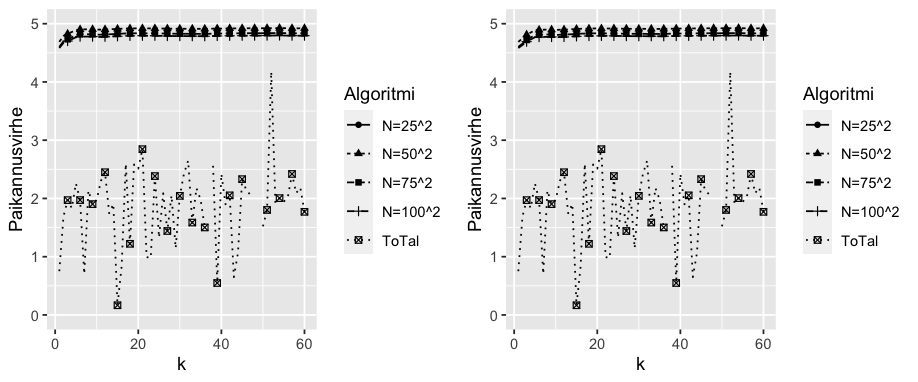
\includegraphics[width=15cm]{prior_likelihood}
\caption{Priori- ja uskottavuusotanta. Ei uudelleenotantaa.}
\label{fig:prior-likelihood}
\end{figure}

Koska ehdotusjakaumalla ei juurikaan ollut vaikutusta tuloksiin, valittiin seuraavaan vaiheeseen muodoltaan yksinkertaisempi uskottavuusotanta. Uskottavuusotantaa käyttäen vertailtiin nyt joka iteraatiolla suoritettavaa uudelleenotantaa (bootstrap) sekä adaptiivista uudelleenotantaa, joka suoritettiin aina, kun effektiivinen otoskoko \(N_{eff}<2N/3\). Tulokset on esitetty kuvassa \(\ref{fig:eachstep-adaptive}\) sekä osana taulukkoa \(\ref{tab:paikannusvirheet}\). Uudeeleenotantamenetelmän valinta ei vaikuta tuloksiin paikannusvirheen suhteen, mutta kuten oletettua, on adaptiivinen uudelleenotanta nopeampi. Nyt myös partikkelien määrän lisääminen parantaa selkeämmin paikkannustarkkuutta ja \(N=100^2\) partikkelilla saavutetaan jo haluttu alle metrin paikannustarkkuus.

\begin{figure}[H]
\centering
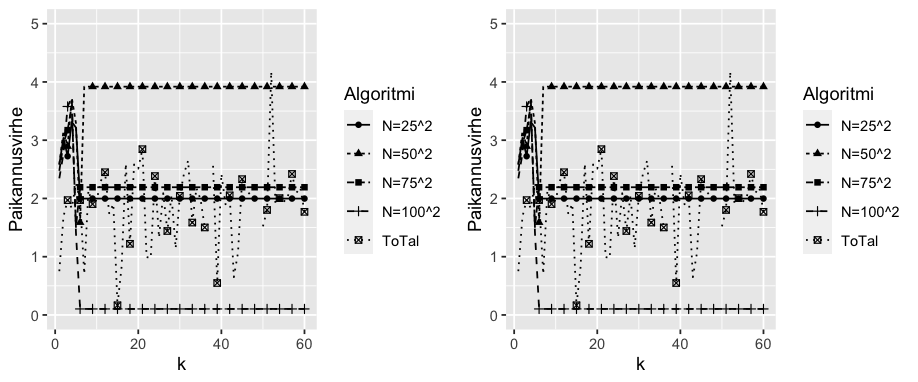
\includegraphics[width=14.5cm]{eachstep_adaptive}
\caption{Jokaisen iteraation uudelleenotanta / adaptiivinen uudellenotanta.}
\label{fig:eachstep-adaptive}
\end{figure}

\newpage

Kuvissa \ref{fig:noresample_maps} ja \ref{fig:resample_maps} esitetään partikkelien jakauma sijainnin suhteen kartalla ajanhetkinä \(k=\{1,3,5,10\}\). Punaiset ympyrät kuvaavat vastaanottimia, sininen neliö testilaitteen todellista sijaintia ja mustat ympyrät partikkelien sijainteja. Molemmat kuvat esittävät uskottaavusotannalla saatuja tuloksia, kun \(N=100^2\). Edellisessä kuvassa \ref{fig:noresample_maps} ei ole käytetty uudelleenotantaa. Vaikka partikkelien painoja ei kuvassa olekaan otettu huomioon, on kuvasta helppo huomata otoskoon ehtymisen ongelma. Jälkimmäisessä kuvassa \ref{fig:resample_maps} on käytetty adaptiivista uudelleenotantaa, joka on suoritettu aika-askelilla 1\textendash 6. Tämä ratkaisee otoskoon ehtymisen ja aika-askeleella \(10\) kaikki partikkelit approksimoivat haluttua sijaintia.

\begin{figure}[h]
\centering
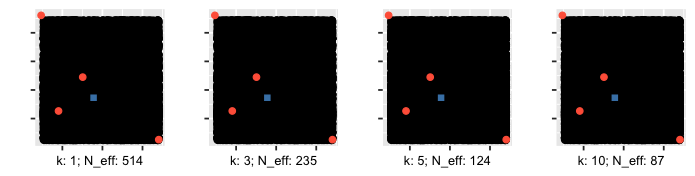
\includegraphics[width=14cm]{SIS_likelihood_maps}
\caption{Partikkelikartta. Ei uudelleenotantaa.}
\label{fig:noresample_maps}
\end{figure}

\begin{figure}[h]
\centering
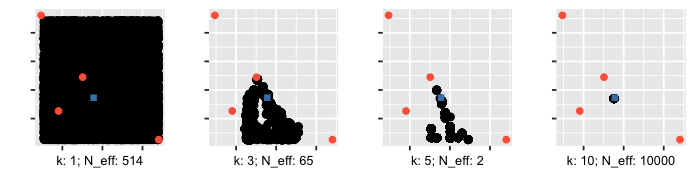
\includegraphics[width=14cm]{SIR_likelihood_maps}
\caption{Partikkelikartta. Adaptiivinen uudelleenotanta.}
\label{fig:resample_maps}
\end{figure}

\def\arraystretch{1.25} 
\begin{table}[H]
\centering
\begin{tabular}{|l|l|l|l|}
\hline
Algoritmi & $N$ & Paikannusvirheen ka. (m) & Keston ka. (s)\\
\hline
ToTal & - & $2.15$ & 0.001\\
SIS/Priori & $25^2$ & 5.31 & 7.91\\
SIS/Priori & $50^2$ & 4.91 & 19.81\\
SIS/Priori & $75^2$ & 4.82 & 46.02 \\
SIS/Priori & $100^2$ & 4.78 & 81.83 \\
SIS/Uskottavuus & $25^2$ & 5.31 & 7.42\\
SIS/Uskottavuus & $50^2$ & 4.90 & 19.85\\
SIS/Uskottavuus & $75^2$ & 4.82 & 45.94\\
SIS/Uskottavuus & $100^2$ & 4.78 & 82.02\\
Bootstrap/Uskottavuus & $25^2$ & 2.08 & 8.64\\
Bootstrap/Uskottavuus & $50^2$ & 3.81 & 21.55\\
Bootstrap/Uskottavuus & $75^2$ & 2.24 & 45.88\\
Bootstrap/Uskottavuus & $100^2$ & 0.33 & 82.24\\
SIR/Uskottavuus & $25^2$ & 2.08 & 7.30\\
SIR/Uskottavuus & $50^2$ & 3.81 & 18.59\\
SIR/Uskottavuus & $75^2$ & 2.24 & 42.11\\
SIR/Uskottavuus & $100^2$ & 0.33 & 79.64\\
\hline
\end{tabular}
\caption{Paikannusvirheet sekä suoritusajat}
\label{tab:paikannusvirheet}
\end{table}

Tuloksista huomataan, että uskottavuusotannalla ja uudelleenotannalla SMC-menetelmät tuottavat esitetyssä koeasetelmassa halutun tarkkuuden. Tarvittavalla määrällä partikkeleita tässä käytetyt SMC-algoritmit ovat kuitenkin aivan liian hitaita tuotantokäyttöön. Vaikka algoritmit pystyvät tuottamaan hitaimmillaankin noin sijainnin sekunnissa, pitää käytännön toteutuksessa sijainteja laskea joka sekunti sadoista paikantimista. Todennäköisesti yksinkertaisin tapa saavuttaa haluttu alle metrin paikannustarkkuus nopeammalla laskennalla on lisätä triangulaatio-paikannukseen jokin laskennallisesti kevyempi suodin, esimerkiksi EKF-suodin.

Koeasetelma toimi kuitenkin hyvänä konseptin todennuksena, sillä käytetyissä SMC-toteutuksissa on useita parannuskohteita. Ensinnäkin algoritmi voidaan toteuttaa täysin \texttt{data.table}-kirjaston avulla tai kokonaan R-ohjelmointikieltä tehokkaammilla ohjelmointikielillä. Toiseksi partikkelien määrää saattaa olla mahdollista laskea paikannustarkkuutta menettämättä käyttämällä parempia malleja. Koeasetelmassa käytetty havaintomalli (\ref{havaintomalli}) on erityisesti kohinan osalta hyvin \textit{ad hoc} -tyyppinen malli. Mallia on mahdollista parantaa esimerkiksi lisämittauksista kerätyn vastaanotindatan avulla. Lisäksi tilamallia (\ref{tilamalli-liikkuva}) pitää testata liikkuvalla lähettimellä, jotta eri paikannusalgoritmien erot tulevat näkyviin myös paremmin todellista käyttötilannetta vastaavassa koeasetelmassa.

\hypertarget{lopuksi}{%
\chapter{Lopuksi}\label{lopuksi}}

Tässä tutkielmassa on esitetty pääpiirteittäin SMC-menetelmien teoria Bayesilaisessa tilastotieteellisessä viitekehyksessä. Lisäksi tutkielmassa on käyty läpi uudelleenotantaa efektiivisen otoskoon perusteella hyödyntävä SIR-suodinalgoritmi. Lopuksi tutkielmassa on tarkasteltu SIR-algoritmin parametrien valintaan, suorituskykyyn sekä konvergenssiin liittyviä tuloksia.

Tutkielmassa on lisäksi tarkasteltu miten eri valinnat vaikuttavat algoritmin suorituskykyyn yksinkertaisen mutta kattavan ja todelliseen ongelmaan sekä dataan perustuvan paikannusesimerkin avulla.

\hypertarget{liitteetfollowed-by-a-chapter}{%
\chapter{\texorpdfstring{Liitteet\texttt{(followed\ by}\# A chapter`)}{Liitteet(followed by\# A chapter`)}}\label{liitteetfollowed-by-a-chapter}}

Konvergenssituloksen \ref{} nojalla kyseinen varianssi \(\sigma^2 \rightarrow \lim 0\), kun \(N \rightarrow \inf\).

  \bibliography{packages.bib,lahteet.bib}

\end{document}
